
\documentclass{article}
\usepackage[utf8x]{inputenc} 
\usepackage{amsmath,bm}
\usepackage{float}
\usepackage[english]{babel}
\usepackage{natbib}
\usepackage{booktabs}
\usepackage{setspace}\doublespacing
\setlength{\parskip}{0.5em}
\usepackage[left]{lineno}\linenumbers
\usepackage[a4paper, total={6in, 8in}]{geometry}
\usepackage{isomath}
\usepackage{amsmath}
\usepackage{mathtools}
\usepackage{longtable}
\usepackage[font={footnotesize,it}]{caption}
\usepackage{rotating}
\usepackage[colorinlistoftodos]{todonotes}


\begin{document}

\begin{center}
\large
\textbf{Social environments and their eco-evolutionary dynamics: from density regulation to frequency-dependent selection}
\end{center}

\begin{center}
	Yimen G. Araya-Ajoy\textsuperscript{1,2}, Myranda Murray\textsuperscript{1},  Bernt-Erik Sæther\textsuperscript{1}, Jonathan Wright\textsuperscript{1}
\end{center}

\bigskip
\noindent \textsuperscript{\textbf{1}} Centre for Biodiversity Dynamics (CBD), Department of Biology, Norwegian University of Science and Technology (NTNU), N-7491 Trondheim, Norway.

\noindent \textsuperscript{\textbf{2}} Corresponding author, email address: yimencr@gmail.com

\bigskip
\noindent \textbf{Running title}:  Social environments and their eco-evo feedbakcs

\bigskip
\noindent \textbf{Type of article}: Synthesis

\bigskip
\noindent \textbf{Keywords}: density-dependent selection, multiple regression, individual-based simulations, social evolution


\newpage
\section{Abstract}
Social interactions are key determinants of the equilibrium density and mean phenotype of populations. Density regulation and frequency-dependent selection can be seen as two extremes of a continuum of effects of social interactions on the eco-evolutionary dynamics of populations. This continuum  describes how much the effect an individual has on the fitness of others depends upon its phenotype, and how much the effects on fitness an individual experiences due to intraspecific interactions depends upon its own phenotype. We use individual-based models to simulate scenarios along this continuum, and analyze the outcomes using a set of multiple regressions designed to disentangle social effects causing temporal variation in population mean fitness from those causing individual differences in fitness. We discuss the links between these different statistical estimates and eco-evolutionary theory concerning the factors determining the equilibrium size and mean phenotype of populations. This synthesis aims to stimulate more focused empirical investigations by connecting specific theoretical components of eco-evolutionary dynamics with standard statistical analyses allowing the quantification of how the social environment affects an individual's fitness and its consequences on population growth and evolutionary change. 

\newpage
\section{Introduction}
 The realization that evolutionary change can affect demographic processes relatively fast has encouraged theoreticians to develop evolutionary models accounting for the feedback between population dynamics and phenotypic evolution \cite[reviewed by][]{Pelletier2009, Hendry2018, Govaert2019}. The basic feature of this feedback is that evolutionary change alters the ecological setting for selection, through its effects on the demographic and phenotypic characteristics of populations, which in turn affects the rate and direction of evolutionary change. Different modeling traditions have been used to address this issue, all sharing the common goal of incorporating these environmental feedbacks on the evolutionary dynamics of phenotypes \citep{Heino1998, Lion2018}. These approaches have provided a variety of insights into the processes determining the links between the equilibrium size of populations and their equilibrium mean phenotype \citep{MacArthur1962, Boyce1984, Charlesworth1994, Abrams1993, Mylius1995, Lande2009a, Engen2020}. However, their diversity and mathematical complexity may be an obstacle for many empiricists in need of a conceptual framework that is both accessible and statistically applicable to natural populations. We thus synthesize key components of these eco-evolutionary theories providing a statistical decomposition of how the characteristics of the social environment affect the fitness of individuals and its consequences for the equilibrium size and mean phenotype of populations. 
 
 We refer to the social environment as the number and phenotypes of individuals creating the ecological context of selection for other individuals. Competitive and cooperative interactions shape the strength of density regulation and phenotypic selection \citep{Lack1954, Haldane1956, West-Eberhard1979, frank1998foundations}, making the interaction between individuals and their social environment a key mediator of the eco-evolutionary dynamics of populations (Box 1). Phenotypes mediating social interactions have the potential to affect population dynamics and/or phenotypic evolution whenever the fitness of an individual is affected by its social environment \citep{Wolf1999SocialSelection, Travis2013}. We can imagine a continuum stretching between two conceptual extremes (Figure 2). At one end we can envision density regulation (from population ecology, Figure 2A) where the effects of density on fitness are assumed to be independent of an individual's phenotype. Whilst at the other end lies frequency-dependent selection (Figure 2H), where the frequency of a phenotype in a population affects its fitness. Most effects of social interactions on the eco-evolutionary dynamics of populations lie somewhere between these two extremes, whenever the impact an individual has on the fitness of others depends upon its phenotype and/or the changes in fitness that an individual experiences due to intra-specific interactions depends upon its own phenotype. 
 
We can make distinction between theories which, in their inception, were more focused on understanding the effect on eco-evolutionary dynamics of the number of individuals in the social environment versus approaches more focused on the effects of the phenotypic and genetic characteristics of the social environment. On the one hand, theory on density-dependent selection was one of the first attempts to unite the fields of population ecology and population genetics, suggesting that fitness of a genotype is not constant but depends on population size \citep{MacArthur1962, Anderson1971, Charlesworth1971}. Considerable theoretical and empirical work has shown that density-dependent selection is an important driver of the variety of life history strategies observed in nature and a key determinant of the relationship between phenotypic variation and the carrying capacity of populations \citep{Boyce1984, Mueller1991, Charlesworth1994,Travis2013, Joshi2001, Engen2013, Wright2018, Engen2020}. On the other hand, social evolution theory has a long tradition focusing on understanding how the phenotypic and genetic characteristics of an individual's social environment can affect short-term evolutionary change \citep{Hamilton1964a, frank1998foundations, Wolf1999SocialSelection, Queller1985a, Queller2017} and long-term equilibrium strategies \citep{MaynardSmith1982, McGill2007}. This framework has further our understanding on how the evolution of the social environment feeds back onto the patterns of phenotypic selection, specially when social interactions are frequency dependent \citep{West-Eberhard1979, QUELLER1984, Araya-Ajoy2020}. 

The eco-evolutionary implications of frequency-dependent selection have been acknowledged since the early mathematical formulation of evolutionary population genetics \citep{Fisher1930, Wright1948}, and quantitative genetic models have further corroborated its importance on determining evolutionary outcomes and the mean fitness of populations \citep{Lande1976, Lande2007, Svensson2018, Engen2020}. Frequency-dependent selection has been used as term describing many different processes (Box 2), but all have in common that the fitness of a phenotype varies with its frequency in the population. There has been long-standing acknowledgment by theoretical population geneticists of the close links between frequency- and density-dependent selection and their intertwined role in the evolutionary dynamics of density regulated populations \citep{Smouse1976, Anderson1983, Heino1998, Joshi2001}. However only until recently, the links between density- and frequency- dependent selection have been dealt with explicitly in a quantitative genetics framework. \cite{Engen2020} have shown how the evolutionary outcome of the joint dynamics of population sizes and phenotypic evolution depends on the interaction between frequency- and density-dependent selection. This work implies that if the mean phenotype in the population modulates the strength of density regulation (Figure 2B), then frequency- and density-dependent selection are extrinsically linked (Figure 2F) and jointly determine the expected equilibrium size and mean phenotype of a population.
 
 A key feature of the eco-evolutionary feedbacks caused by the evolution of the social environment is that they are mediated by phenotypes that have fitness effects on individuals other than the actor. The evolutionary consequences of such phenotypes (Figures 2C and D) is the focus of quantitative genetics theory on social evolution \citep{frank1998foundations, Araya-Ajoy2020}. This theoretical framework has a statistical component based upon methods for empirically studying deterministic quantitative genetics theory to predict evolutionary responses to selection \citep{Robertson1966, Lande1976, Lande1979, Lande1983}. A key tool in this framework is multiple regression, which has been widely used to estimate direct and indirect effects of phenotypes on fitness \citep{Kingsolver2011}. In a social evolution context, this approach is used to study the effects of the social environment of an individual on its fitness. The magnitude of these effects are measured as social selection gradients \citep{Wolf1999SocialSelection} either parameterized as a neighbor-modulated approach \citep{Okasha2006} or in a contextual analyses of fitness \citep{Heisler1987, Goodnight1992}. Furthermore, multiple regression has been used to study density regulation by estimating how density affects fecundity and/or survival \citep{Araya-Ajoy2021, Saether2021} and as a conceptual tool to understand the role of frequency-dependence in social evolution \citep{Araya-Ajoy2020, Westneat2012a}. The multiple regression approach thus constitutes a key conceptual and empirical tool to link processes relating phenotypic evolution with population dynamics. 

In the next section we provide a statistical decomposition of the various ways in which the fitness of individuals is affected by their social environment using multiple regression equations. In doing so, we aim to stimulate much needed empirical research using readily available statistical tools that will enable critical tests of specific theoretical predictions in the context of eco-evolutionary dynamics. We describe a set of scenarios increasing in complexity, starting from a scenario of simple density regulation all the way until its interaction with the mean phenotype in the population causes density- and frequency-dependent selection to become intrinsically linked. We present the multiple regression equations that can be used to analyze each scenario empirical and then rearrange them to highlight how one can statistically determine the contribution of different social process to the equilibrium size and mean phenotype in the population. We further use individual based models (Box 3) to simulate data representing these scenarios and analyze them with the corresponding multiple regression equations. In doing so, we confirm that the observed equilibrium phenotypic value and population size in each simulation can be calculated based upon the parameter values estimated in the multiple regression analyses. The basic features of the individual-based simulation are that density regulation causes the average fitness of the population to decreases with population size and that an individual's fitness can be affected by its own phenotype and the phenotype of the other individuals in the population. Interactions between these different processes will have direct consequences on the equilibrium population size and mean phenotype. 


\section{A continuum of (simulated) scenarios}
\subsection{Density regulation (S1)}
Here we refer to density regulation to situations were population growth rates are regulated by the density of a population. Our first scenario, describes a strictly ecological feedback were only density regulation determines the equilibrium size of populations. This is the simplest and most fundamental effect of the social environment on an individual's fitness \citep{Brook2006}. In this scenario (S1) an individual's phenotype does not affect its fitness and the effect of the social environment on the fitness of individuals depends only on the number of individuals in the population, implying that evolution and population dynamics are uncoupled. The strength of density regulation could reflect the degree of interference competition affecting the number of recruits produced by a flock of birds breeding in a newly colonized island. As population size increases females are able to produce fewer recruits because there are fewer resources for everyone. The multiple regression equation describing this scenario is:

\begin{equation} \label{eq: fitness1}
\bm{w}=\beta_{0} +\beta_{n} \bm{n}  +  \bm{\epsilon}.
\end{equation}

\noindent Here $\bm{w}$ is the absolute fitness of individuals, $\beta_{0}$ is the expected average individual fitness when the population size is zero or very small. In the context of a multiple regression, $\beta_{0}$ is a constant estimated as the intercept in the model, if population size is not mean centered. How an increase of one individual in the population will affect the fitness of all individuals is described by the density regulation coefficient $\beta_{n}$, where $\bm{n}$ is a vector of population sizes experienced by each individual. All other 'unmeasured' processes affecting the fitness of individuals in a given year are represented by $ \mathbf{\epsilon}$. In a statistical sense, this constitutes the 'residual' unexplained variation in individual fitness. It is important to note here that $\mathbf{w}$ and $\mathbf{e}$ vary among individuals and among reproductive episodes, while only $\mathbf{n}$ varies among reproductive episodes (e.g. years). This equation is thus describing the fitness of individuals across many breeding episodes.

A key consideration here is what fitness measure to use. When quantifying the dual role of social interactions on phenotypic evolution and population dynamics, it is crucial to use a demographically relevant measure of individual fitness that connects to annual population-level changes. Hence, the fitness measure we use throughout this study is annual individual fitness, which is survival plus half the number recruits produced by each individual \textit{i} in a given year \citep{Saether2015}. Summing this episodic fitness measure across all individuals will be equal to the expected size of a population in the next year or breeding episode (equation  \ref{eq:fitness measure}). 

\begin{equation} \label{eq:fitness measure}
n_{t+1}=\sum \bm{s} + \frac{\bm{r}}{2}= \sum w=\bar{w}n_{t}, 
\end{equation}

\noindent where  $\bm{s}$ is a vector of values describing whether individuals survived or not to the year $t+1$ and $\bm{r}$ is a vector of the number of recruits produced by each individual in year t. While the mean fitness of the population $\bar{w}$ in a give year multiplied by the population size in that year $n$ equals the expected population size at time $n_{t + 1}$. When the mean of this fitness measure is more than one, populations are expected to grow, and if it is less than one they are expected to decline.

The expected equilibrium population size can thus be estimated by rearranging the relevant coefficients of equation \ref{eq:fitness1} describing how individual fitness is affected by population size :

\begin{equation}\label{eq:equilibrium}
\hat{n}=\frac{1-\beta_{0}}{\beta_n}. 
\end{equation} 

\noindent The equilibrium size of the population is therefore defined by the strength of density regulation, estimated as $\beta_n$ and the fitness of individuals when the population is very small, estimated as $\beta_0$. We used the individual based simulations to show how the strength of density regulation affects the equilibrium population size (density regulation; Figure \ref{fig:sim2}A) and the equilibrium size can be estimated used the regression parameters (Table 2). The simulations clearly show that varying the strength of the coefficient determining density regulation has direct consequences on the equilibrium population size (\ref{fig:sim2}A.i), through its effects on the relationship between population size and mean fitness (Figure \ref{fig:sim2}A.iii). In this scenario there was no effect of the phenotype on fitness, as expected, therefore the mean phenotype in the population does not change across time (Figure \ref{fig:sim2}A.ii). 

\subsection{Hard selection (S2)}
This scenario (2) extends on the previous one and focuses on a situation where the phenotype of an individual has a direct effect on its own fitness. We refer to this relation between phenotype and fitness as "hard selection" \citep{Wallace1975, Bell2021} because the effect of an individual's phenotype on its fitness is independent of its social environment (i.e. is frequency and density independent). This results in that phenotypic evolution affects the equilibrium size of the population through its effects on mean fitness. Adaptation through phenotypic evolution results in that the average individual has a higher reproductive success and the size of the population increases. We can think of body size as the focal phenotype and selection favoring larger individuals because they can obtain larger quantities of food (e.g. larger birds can capture the more numerous larger prey items). The mean fitness of the population increases because individuals can produce more offspring as the average individual can access more resources. 

The multiple regression equation for the statistical analyses for this scenario is:

\begin{equation} \label{eq:fitness1}
\bm{w}=\beta_{0} +\beta_{n} \bm{n} + \beta_{z} \bm{z} + \beta_{q} \bm{z}^2 +  \bm{\epsilon}.
\end{equation}

We now include the effect of an individual's phenotype on fitness assuming a quadratic relationship between the trait and fitness. We thus include the coefficients $\beta_{z}$ and $\beta_{q}$ describing the linear and quadratic components of the relationship between the phenotypic value ($\bm{z}$) and absolute fitness ($\bm{w}$). In a scenario of hard selection evolutionary change is expected to move the mean phenotype of the population towards the optimum phenotype. The optimal phenotype is defined here as the phenotypic value that confers the highest fitness ($\theta$). This is described by the parameters $\beta_{z}$ and $\beta_{q}$. When populations are perfectly adapted to their environment the mean phenotype is equal to the optimal phenotype. Under this simulated scenario (2) the value for the mean phenotype $\hat{z}$ that equals the optimal phenotype ($\theta=\hat{z}$) is the equilibrium phenotype,
 
\begin{equation}
\theta=\hat{z}=\frac{-\beta_{z}}{2\beta_{q}}
\end{equation}

\noindent Expressing $\theta$ as function of $\beta_{z}$ and $\beta_{q}$, and substituting it into equation \ref{eq:fitness1}, we can infer the equilibrium population size ($\hat{n}$) based upon the estimates of a linear regression:

\begin{equation}\label{eq:equilibrium1}
\hat{n}=\frac{1-\beta_{0}- \beta_{z}\hat{z} - \beta_{q}\hat{z}^2}{\beta_n}. 
\end{equation}

In the early formulations of Wright's adaptive topography \citep{Wright1931}, evolution by natural selection was assumed to increase the mean fitness of the population, implicit in this argument is that size of the population will increase. We used the individual-based simulations for scenario (S2) to show this by varying the strength of directional selection and demonstrate how it results in different equilibrium phenotypes and its consequences to the equilibrium population size (Figure \ref{fig:sim2}B). Here we represent the situation were hard selection increases the average fitness of the population when the population size is small, leading to a larger population size at equilibrium. Phenotypic evolution here thus shapes the elevation of the relationthsip between population size and mean fitness (Figure \ref{fig:sim2}B.iii).  For instance different types of change in the environment, such as alternative new types of food resources becoming available, could lead to selection for alternative phenotypic values as each new foraging phenotype value evolves to be best suited to exploiting one particular type of new resource. Contrasting profitabilities, in terms of the fitness costs of producing the different phenotypes versus the fitness benefits of exploiting the different new resources, could affect the mean fitness of populations producing contrasting equilibrium population sizes despite similar levels of density regulation.

 
\subsection{"Hard" social selection or frequency-dependent selection I (S3)}
The next scenario (S3) represents situations were the fitness of an individual not only depends upon its own phenotype, but also upon the phenotype ($\bar{z}$) of the indivudals in its social environment (figure \ref{fig:selection}C). For example, as the mean body size of individuals in the population increases, the amount of resources available to each individual decreases due to contest and scramble competition, because individual fitness is more negatively affected by the presence of larger competitors. We assume that individuals interact at random with equal probability with all other individuals in the population (“playing the field”, \cite{MaynardSmith1982}), and thus the effects of the social environment on individual fitness can be captured by including the effect of the population mean phenotype $\bar{z}$ on the fitness of individuals. This effect can be included as another coefficient ($\beta_{\bar{z}}$) in the multiple regression equation as:  

\begin{equation} \label{eq: socialselection}
\bm{w}=\beta_{0} +\beta_{n} \bm{n} + \beta_{z} \bm{z}+ \beta_{\bar{z}} \bar{\bm{z}}+ \bm{e}.
\end{equation}

This new term is similar to what has been refer to as a social selection gradient. Social selection gradients usually quantify the effect of the phenotypes in the social environment on the relative fitness of an individual within a given breeding episode \citep{Wolf1999SocialSelection}. In this context, it is assumed that social fitness effects influence evolutionary changes in the mean phenotype in the population, but they do not affect the growth of populations. Similar to `soft' selection \citep{Wallace1975, Bell2021}, this type of social selection has no effect on the mean fitness of the population \citep{Goodnight1992}, and thus no consequences in terms of variation in population size (Figure 2D). However, as we show here, the effect of the phenotype of the average individual in the population on the absolute fitness of other individuals is expected to affect the mean fitness in the population. The phenotypic effects of an individual on the survival and reproduction of others can thus influence the mean fitness of the population (shown as black dots in Figure 2C) in a similar way to density regulation (Figure 2A). This type of effect of the social environment on fitness also results in that the fitness of the different phenotypes is dependent on their frequency, and can thus be consider a type of frequency-dependent selection (Box 2). This type of "hard" social selection will partly define the relationship between the mean phenotype in the population and its mean fitness \citep{Lande1976}, linking the evolutionary trajectory of the phenotype with the dynamics of population size.

\noindent Rearranging equation \ref{eq:equilibrium1} to find the equilibrium population size:

\begin{equation}
\hat{n} = \frac{1-\beta_{0} - (\beta_{z} + \beta_{\bar{z}} +  \beta_{q}\bar{z})\hat{z}}{\beta_{n}},
\end{equation}

\noindent we can see that equilibrium population size $\hat{n}$ depends upon both the direct effect of the phenotype on fitness and the indirect effects that the phenotype has on the fitness of others ($\beta_{z} + \beta_{\bar{z}})$. This follows previous work showing that the effect of the mean phenotype of the population on average fitness is defined by two distinct processes \citep{Engen2020, Lande2007, Lande1976}. On the one hand it is determined by the effect of an individual's own phenotype on its fitness ($\beta_{z}$), and on the other by the effect that the phenotype of the other individuals in the social environment has on an individual's fitness ($\beta_{\bar{z}}$).

A key realization of early population genetics models was that under many types of frequency-dependent selection, evolution will not always maximize the mean fitness in the population \citep{Fisher1930, Wright1948}. We exemplify this using the individual-based simulations (Figure \ref{fig:sim2}C). When the direct effect of phenotypes on fitness is positive and there is also a positive social fitness effect ($\beta_{z}>0$ and $\beta_{\bar{z}}>0$), the equilibrium population size is larger as compared to a case where the phenotypes of others have a negative effect on individual fitness ($\beta_{z}>0$ and $\beta_{\bar{z}}<0$). The first case may represent a (cooperative) social phenotype that allows each individual to utilize resources more efficiently (e.g. cooperative foraging in social spiders, \cite{Majer2018}). This maximises individual fitness whilst freeing up more resources for use by other individuals in the population, thus increasing average fitness in the population and the population carrying capacity (Figure \ref{fig:sim2}C, green line). The other case could represent a competitive phenotype (e.g. body size effects in foraging competition in fish, \cite{Ward2006}), which allows each individual to monopolize more resources while reducing the resources available for other individuals in the population (Figure \ref{fig:sim2}C, red line), thus decreasing average fitness of the population and its carrying capacity. Therefore, even with similar equilibrium phenotypes (Figure \ref{fig:sim2}C.ii) the equilibrium population size can be quite different (Figure \ref{fig:sim2}C.i) depending upon the strength and direction of 'hard' social selection and its consequences for the elevation of the population size fitness relation (Figure \ref{fig:sim2}C.iii). 

\subsection{Phenotype-dependent density regulation (S4)}
These scenarios of social selection alongside the (additive) effects of density regulation (Figure \ref{fig:sim2}C) could be seen as unrealistically simple. This is because when the mean phenotype in the population affects the amount of resources available, it is likely that is in interaction with the number of individuals present in the population (depicted in Figure 2B). In other words, it is more likely that there is phenotype-dependent density regulation (figure \ref{fig:selection}F). We could think about this as the biomass (${n\bar{z}}$) of the population affecting individual fitness via competition for a given supply of food resources. This scenario extends the linear regression equation once more to include the coefficient $\beta_{n \bar{z}}$, describing phenotype-dependent density regulation as the effect on fitness of the interaction between population size $\bm{n}$ and the mean phenotype $\bar{\bm{z}}$ in the population: 

\begin{equation} \label{eq: PDDR}
\bm{w}=\beta_{0} +\beta_{n} \bm{n} + \beta_{z} \bm{z}+ \beta_{\bar{z}} \bar{\bm{z}} + \beta_{n\bar{z}} \bm{n} \bar{\bm{z}}  +  \bm{e}.
\end{equation}

While the "frequency" of a genetoype is clearly involved in this process, we do not include this as a type of frequency-dependent selection because it is not "pure" frequency-dependent selection but reflects how the strength of frequency dependence is modified by the number of indivdiuals in the population. We can think about this processes as density regulation working via a new quantity determined by the product of the number of individuals and the mean phenotype in the population $\bm{n}\bar{\bm{z}}$ \citep{Engen2020}. However, for the purposes of the multiple regression analysis, the inclusion of the interaction term ($\beta_{n\bar{z}}$) defines the coefficient ($\beta_{n}$) as the relationship between population size and fitness when the mean phenotype of the population is zero. The coefficient $ \beta_{\bar{z}}$ then represents the effect of the average phenotype in the social environment on individual fitness when the population size is zero. 

Rearranging equation \ref{eq: PDDR}, we can see that the expected equilibrium population size ($\hat{n}$) now depends upon the (equilibrium) population mean phenotype ($\hat{z}$) in yet another way:

\begin{equation}
\hat{n} = \frac{1-\beta_{0}-(\beta_{z}  + \beta_{\bar{z}} + \beta_{q}\hat{z})\hat{z}}{(\beta_{n} +  \beta_{n\bar{z}} \hat{z})},
\end{equation}

\noindent because the strength of density regulation is now also moderated by the mean phenotype in the population as a function of the coefficient  $\beta_{n\bar{z}}$. 

The concept of phenotype-dependent density regulation is at the core of the early theoretical models focusing on frequency dependent interactions in density regulated populations \citep{Clarke1972, Anderson1983}. As opposed to the early models of evolution in density regulated populations were all genotypes contributed equally to density regulation, in these models different genotypes have a different contribution to density regulation. The eco-evolutionary dynamics of phenotype dependent contributions to density regulation has been recently studied in a quantitative genetic framework by \cite{Engen2020}. Using the individual-based simulations we show that this additional way that social traits can mediate the strength of competition can increase or decrease the strength of density regulation, further affecting the equilibrium size of the population (Figure \ref{fig:sim2}D.i). Phenotype dependent density regulation thus affect the equilibrium size of the population throught its effect on the slope of the population size-mean fitness relationship (Figure \ref{fig:sim2}D.iii). For instance, in cases where density regulation occurs through the effect of individual biomass \citep{Owen-Smith2002}, an increase in the number of heavier individuals (larger body mass) will reduce the amount of resources disproportionately more \textit{per capita}, as compared to an increase in the number of lighter individuals (smaller body mass). In this scenario, even with the same equilibrium phenotype (Figure \ref{fig:sim2}D.ii), the equilibrium population size depends on how the mean phenotype influences the strength of density regulation (Figure \ref{fig:sim2}D.iii). 

 \subsection{Density-dependent selection (S5)}
 Thus far we have described scenarios were the fitness of an individual is affected by its own phenotype and the number and phenotypes of the individuals in its social environment. However, we have assumed that the relationship between an individual's phenotype and its own fitness is not dependent the social environment. Here we focus on a scenario where the effect of population size on individual fitness depends on an individual's own phenotype. This could represent a scenario were smaller body size phenotypes are favoured in low densities due to the their higher reproductive rates that come at the expense of investment somatic growth, whereas at high population densities larger individuals are favoured due to their abilities to monopolize resources despite of their lower reproductive rates. For simplicity, we present this scenario without including frequency-dependent selection. The regression equation thus focuses only on the inclusion of the coefficient $\beta_{nz}$ (Figure \ref{fig:surface}A), thereby modelling the interaction effect between an individual's phenotype and population size on fitness:

\begin{equation} \label{eq: DDRS}
\bm{w}=\beta_{0} +\beta_{n} \bm{n} + \beta_{z} \bm{z}+  \beta_{zn} \bm{zn}  +  \bm{e}.
\end{equation}

\noindent Density-dependent selection closely connects the equilibrium mean phenotype and the equilibrium population size of the population, because now the equilibrium phenotype in the population depends upon population size:

\begin{equation} 
\hat{z}=\frac{-(\beta_{z}+\beta_{zn}\hat{n})}{2\beta_{q}},
\end{equation} 

and the equilibrium size of the population depends upon the equilibrium phenotype:

\begin{equation} \label{eq: equilibrium DDRS}
		\hat{n} = \frac{1-\beta_{0}-(\beta_{z}  + \beta_{q}\hat{z})\hat{z}}{(\beta_{n} +  \beta_{zn} \hat{z})}.
\end{equation}

\noindent Note that the equilibrium phenotype in the population affects the equilibrium population size here in a different way than previous results (above), because the effect of population density on an individual's fitness depends upon its own phenotype ($\beta_{zn} \hat{z}$). 

Fluctuating selection associated to changes in the size of populations has been at the core of evolutionary theory explaining the observed diversity of life histories in nature \citep{Pianka1970,macarthur1967theory, Boyce1984, Mueller1991, Engen2013}. A classic theoretical result \citep{MacArthur1962, Engen2013} shows that when selection is density-dependent then evolution is predicted to maximize the function describing the expected population size ($\hat{n}$). According to these models, evolution is expected to favor the phenotypic value that increase the numerator of equation \ref{eq: equilibrium DDRS} and the decrease its denominator. This parallels arguments about the adaptive topography of populations, where evolution should maximize the mean fitness of populations \citep{Wright1931}. However as we have described in previous scenarios, this is not necessarily the case when selection is frequency dependent. The inclusion of frequency-dependent selection on the evolutionary models for density regulated populations was partly aimed at explaining that selection under crowded environments will not necessarily lead to a higher mean fitness in the population,  higher carrying capacities and larger population sizes \citep{Clarke1972, Anderson1983, Engen2020}. 

 
\subsection{Frequency-dependent selection III (S6)}
We further focus on a scenario where the optimal phenotype in the population depends on the mean phenotype of the population (S5 Frequency-dependent selection III, depicted in Figure 2G). We explicitly leave density-dependent selection and phenotype-dependent density regulation out in this scenario for the sake of argumentation. Following our body mass example, this scenario might represent situations where smaller body size phenotypes are favoured when most individuals are large due to the ability of smaller individuals to keep breeding and better withstand the negative effects of high competition on somatic maintenance of a larger body. However when the population is composed of mostly smaller individuals, selection favors larger bodies that can out compete for resources the smaller individuals. This scenario may also capture classic behavarioal ecology evolutionary games such as the hawk-dove situation \citep{MaynardSmith1982}. Where the fitness benefits of playing dove depend on the number of hawks in the populations and viceversa. In a continuous trait, this leads to a type of balancing selection that results in a equilbrium mean phenotype or fluctuations around this equilibrium mean phenotype. We distinguish this scenario from scenario 4 and refer to it as frequency-dependent selection III (Box 2), because there is an interactive (as opposed to additive) effect on fitness of an individual's own phenotype and the phenotype of its social environment \citep{Araya-Ajoy2020}. Implicit in these interactive effects is that the shape of the fitness function changes depending on the social environment. This is captured by the coefficient $\beta_{z\bar{z}}$, representing the interaction between an individual's own phenotype and the mean phenotype in the population:  

\begin{equation} \label{eq: FDS}
\bm{w}=\beta_{0} +\beta_{n} \bm{n} + \beta_{z} \bm{z}+ \beta_{\bar{z}} \bm{\bar{z}}  + \beta_{z\bar{z}} \bm{z\bar{z}}  +  \bm{e}.
\end{equation}

\noindent In the presence of pure frequency-dependent selection III, the equilibrium phenotype is not only a function of the quadratic fitness function, but is also affected by the frequency-dependent selection coefficient $\beta_{\bar{z}}z$:

\begin{equation} 
\hat{z}=\frac{-\beta_{z}}{2\beta_{q} + \beta_{z\bar{z}}}.
\end{equation} 

\noindent The frequency dependent coefficient will, in turn, affect the size of the population:

\begin{equation}
\hat{n} = \frac{1-\beta_{0}-(\beta_{z}   + \beta_{\bar{z}})\hat{z} + (\beta_{q} - \beta_{z\bar{z}})\hat{z}^2}{\beta_{n}}.
\end{equation}

\noindent The equilibrium size of the population here will thus be affected by the mean phenotype in the population through three processes: (i) the direct effect of an individual's phenotype on its own fitness (mediated by $\beta_z$ and $ \beta_q$); (ii) the indirect effects on the fitness of other individuals in the population ($\beta_{\bar{z}}$); and (iii) how the direct effect of an individual's phenotype on its own fitness depends upon the average phenotype in the population ($\beta_{z\bar{z}}$). 
 
 Frequency dependent selection is a core component of evolutionary game theory \citep{MaynardSmith1982}. Within this framework it is often assumed that the population size is fixed, and thus for simplicity that the evolutionary dynamics of social interactions do not affect the size of populations and  \textit{vice versa}. However using the individual based simulation we show that this type of frequency dependent selection is also expected to affect the equilibrium population size. Frequency-dependent selection III will affect the equilibrium population size (Figure \ref{fig:sim3}B.i) through its effects on the equilibrium phenotype (Figure \ref{fig:sim3}B.ii). It will only affect the intercept of the relationship between population size and mean fitness, and not the slope (Figure \ref{fig:sim3}B.iii). Importantly, mixtures of density- and frequency-dependent selection (Figure 2H) are probably ubiquitous in natural populations, involving more or less phenotype-dependent impacts on, and responses to, population density. It thus seems important then that empirical studies of frequency-dependence consider how it is associated with and modified by density-dependent effects, and \textit{vice-versa}.

\subsection{Frequency-density-dependent selection (S7)}
Finally we describe a scenario where the optimal phenotype depends upon an interaction between the number of individuals and the phenotype of the average individual in the population (Figure 2F). When focusing on a continuous phenotype, if density regulation is modulated by the mean phenotype of the population, then the effects of density fluctuations on the fitness of individuals depends on the mean phenotype of the population \citep{Engen2020}. Therefore when the optimal fitness depends on the strength of competition then density-dependent selection and frequency-dependent selection are intertwined as pointed out by \cite{Smouse1976} and \citep{Heino1998}. Because the fitness of a phenotype depends on both the number and phenotypes of individuals in their social environment. This would could represent a scenario in which the fitness benefits of a more competitive larger body size depends on the biomass of the population. For instance when the advantages of a larger body size are especially apparent in more competitive environments were most individuals are large and population density is high. When focusing on the multiple regression analyses, we need to further include a three-way interaction ($\beta_{\bar{z}zn}$) capturing the interaction between frequency- and density-dependent selection:

\begin{equation} \label{eq: fullw}
\bm{w}=\beta_{0} +\beta_{n} \bm{n} + \beta_{z} \bm{z}+ \beta_{\bar{z}} \bm{\bar{z}}  +   \beta_{n\bar{z}} \bm{n\bar{z}} +   \beta_{zn} \bm{zn} + \beta_{z\bar{z}} \bm{z\bar{z}}   +   \beta_{zn\bar{z}} \bm{zn\bar{z}} + \bm{e}.
\end{equation}

\noindent We have now reached the most complex form of this regression equation, which includes all of the different parameters discussed (see Table 1 and Figure 2). Here, the coefficient $\beta_{z\bar{z}n}$ captures how the effect of population density on an individual's fitness depends upon the mean phenotype of other individuals in the social environment, and how this social effect, in turn, depends upon the individual's own phenotype (Figure \ref{fig:sim3}C). The equilibrium phenotype of the population thus depends upon the equilibrium population size: 

\begin{equation} 
\hat{z}=\frac{-(\beta_{z}+\beta_{zn}\hat{n})}{2\beta_{q} + \beta_{z\bar{z}} + \beta_{z\bar{z}n}\hat{n}},
\end{equation} 

\noindent and the equilibrium size of the population depends upon the equilibrium phenotype:

\begin{equation}  \label{eq: full}
	\hat{n} = \frac{1-\beta_{0}-(\beta_{z}  +  \beta_{\bar{z}})\hat{z} - (\beta_{q} + \beta_{z\bar{z}})\hat{z}^2 }{\beta_{n} + (\beta_{zn} + \beta_{n\bar{z}}) \hat{z} + \beta_{zn\bar{z}}\hat{z}^2}.
\end{equation}

When the fitness of a phenotype depends upon the mean phenotype in the population and its interaction with the number of individuals, it may not be possible to find an analytical solution for the equilibrium mean phenotype and the population size \citep{Engen2020}. In this scenario, the evolutionary outcome can be an array of combinations of mean phenotype and equilibrium population sizes (Figure \ref{fig:surface}). This complicated dynamic was described in early models of frequency-density dependent models in a population genetics framework. These models were based on the Lotka Volterra formulations for multi-species interactions characterized by a matrix of interaction coefficients describing how the abundances of each species or genotype affects fitness of the other genotypes or species \citep{Clarke1972, Anderson1983}. The three way interaction presented here $\beta_{n\bar{z}z}$ captures similar dynamics but focusing on continuous traits \citep{Engen2020}, explicitly modeling the differential contribution to density regulation of different mean phenotypes, as well as the differential sensitivity to density of the different phenotypes.   

\section{Discussion}
Phenotypic evolution can cause changes in the social environment, in terms of the number of individuals composing it and their phenotypes, these changes will feedback to alter the ecological setting for selection, with cascading effects on density regulation and phenotypic evolution. We show how it is possible to describe the characteristics of this feedback using a set of regression parameters that can be estimated empirically. Reviewing components of eco-evolutionary theory from this perspective, highlights that systematically disentangling the processes creating variation among- and within-reproductive episodes on a measure of fitness that directly links to changes in population size \citep{Saether2015}, it is possible to study different social processes determining the relation between the equilibrium mean phenotype of a population and the number of individuals it can sustain. 

\subsection{Evolution of population size}
Combining individual-based simulations with mathematical descriptions based upon multiple regression parameters, we are able to demonstrate the variety of ways in which phenotypic evolution can affect the equilibrium size of populations. Phenotypic evolution can influence the equilibrium size of populations through social traits affecting density-independent fitness, but also through traits directly involved in how population size affects the density-dependent fitness of individuals. Density-independent evolution influences population size through phenotypic selection shaping the intercept of the function describing population size effects on individual fitness (see Figure \ref{fig:sim2}B.iii \& C.iii). Correspondingly, density-dependent evolution affects density regulation via phenotypic selection shaping the slope of this same population size-individual fitness function (Figure \ref{fig:sim2}D.iii \& \ref{fig:sim3}A.iii). A greater carrying capacity will thus evolve when selection on traits leads to a higher intercept and/or a shallower slope in the population size-individual fitness function. This dichotomy can be seen in equation \ref{eq: full}, where density-independent effects on fitness are grouped in the numerator, whereas density-dependent effects on fitness are grouped in the denominator.

The relationship between the phenotypic characteristics of a population and its density was the focus of early life-history studies framed in terms of \textit{r}- versus \textit{K}-selection \citep{macarthur1967theory}. It is now recognised that we can view such \textit{r}- versus \textit{K}-selection as a particular sub-set of a wider array of patterns of density-dependent selection \citep{Boyce1984, Wright2018, Engen2020}. \textit{r}-selection occurs when populations are at low densities and selection favors higher rates of reproduction, as competition is not constraining the fitness of individuals. Intraspecific competition in \textit{r}-selected species was thus hypothesized to be of 'scramble' type, varying in intensity with fluctuations in the availability of resources \citep{Southwood1977}. In contrast, as populations approach carrying capacity \textit{K}-selection favors traits that enhance an individual's ability to monopolize resources in crowded environments or increase their efficiency of resource utilization \citep{Boyce1984}. If selection favors traits enhancing cooperation and resource efficiency, it will incidentally increase the carrying capacity of populations, fitting the definition of \textit{K}-selection as originally stated by \cite{macarthur1967theory}. One of the earlier criticisms of the \textit{r}- versus \textit{K}-selection framework was that selection under crowded conditions does not necessarily results in higher carrying capacities \citep{Boyce1984}. This criticism partly stemmed the observation that if selection under crowded environments favors traits that result in costly investment by all parties in 'contest' competition, it will decrease the expected equilibrium size of populations \citep{Joshi2001, Engen2020}. Using the multiple regression descriptions of how the social envrionment affects an individuals fitnesss and the individual based simulation we show this distinction by showing how the effect of phenotypic evolution on equilibrium population sizes will be partly determined by the sign and magnitude of the regression coefficients describing how the access to resources in one individual affects the access to resources for others.

  Selection under crowded conditions directly affecting the competitive ability of individuals has been covered in the literature under the concept of ${\alpha}$-selection \citep{Joshi2001}. An explicit distinction can therefore be made between the evolution of strategies increasing tolerance to crowding through higher efficiency in resources use (\textit{K}-selection) versus the evolution of strategies that inhibit the fitness of others when population density is high (${\alpha}$-selection). Early population genetics models of `density-frequency-dependent selection focused on evolutionary dynamics when interacting genotypes have different competitive abilities ($\alpha$) and different $K$ \citep{Clarke1972, Anderson1983}. These models showed how the interaction between density regulation and frequency-dependent selection can lead to resource specialization, potentially increasing the carrying capacity of populations and leading to the maintenance of polymorphisms. More complete formulations of these models have recently been developed using a quantitative genetics framework to study the eco-evolutionary dynamics of populations stochastically fluctuating in size \citep{Lande2007, Engen2020}. This modeling approach provides insights on how the interaction between density- and frequency-dependent selection can result in a variety of combinations of mean phenotypic values and equilibrium population sizes. We illustrate these same biological processes in a non-stochastic environment in order to show how traits can modulate the strength of density regulation when the effect of increasing density on an individual's fitness depends upon the phenotypes of the other individuals in the population (Figure \ref{fig:sim2}D), and/or when the effects of population density on an individual's fitness depends upon its own phenotype (Figure \ref{fig:sim3}A). Whenever these two processes happen at the same time then density- and frequency-dependent selection are intrinsically linked, because the effect of the number of conspecifics and their phenotypes on an individual's fitness also depends upon its own phenotype (Figure \ref{fig:sim3}C). The dynamic equilibrium of the mean phenotype and the size of populations associated to social interactions is thus dictated by phenotype dependent density regulation and how the fitness function is dependent on the number and phenotypes of the individuals in the social environment (frequency-density-dependent selection).  

\subsection{Deterioration of the social environment}
In the early formulations of Wright's adaptive topography \citep{Wright1931}, evolution by natural selection was assumed to increase the mean fitness of the population. However, \cite{Fisher1930} noted that the log mean fitness of populations at equilibrium is expected to fluctuate around 0. He coined the term environmental deterioration to explain tthe "evolutionary stasis" of mean fitness in populations at their equilibrium size, even when natural selection favors traits that increase an individuals own fitness \citep{Slatkin1991}. Environmental deterioration directly relates to the ecological feedbacks caused by the evolution of the social environment and can be thought of as the changes in the social environment counteracting the expected increases in mean fitness caused by the effect of "hard" selection. We can express the change in mean fitness $\Delta \bar{w}$ as a function of changes in the in the number of individuals in the social environment ($\Delta n$) and their mean phenotype $\Delta \bar{z}$ from one generation to the next focusing on the coefficients in equation \ref{eq: fullw}:  

\begin{equation} \label{eq: fisher}
\Delta \bar{w} =  (\beta_{z}\Delta \bar{z}) + (\Delta n\beta_{n} + \Delta \bar{z} \beta_{\bar{z}} + \Delta n \Delta \bar{z} \beta_{n\bar{z}}) + ( \Delta n  \beta_{zn} + \Delta \bar{z} \beta_{z\bar{z}} + \Delta n \Delta\bar{z} \beta_{zn\bar{z}})\Delta \bar{z}.
\end{equation}

We can group these effects on the change in mean fitness in three terms (defined by brackets). The first term groups natural selection processes that are expected to favour traits that maximize an individual's fitness independent of its social environment (Hard social selection). Changes in the mean phenotype solely associated to hard selection ($\beta_{z}\Delta \bar{z}$) are expected to increase the population mean fitness. The second term groups process that can potentially counteract the positive effects on mean fitness of natural selection. For instance, increases in population size due to the effects of hard selection on mean fitness will negatively affect the fitness of individuals due to density regulation $(\Delta n\beta_{n}$). Similarly evolutionary changes favoring phenotypes that positively affect an individual's fitness but negatively affects the fitness of others, will have negative effects on the mean fitness of a population ($\Delta \bar{z} \beta_{\bar{z}}$) canceling the positive effects of hard selection. This effect may be exacerbated if the strength of density regulation is modulated by the mean phenotype in the social environment as in scenario 4. The third term represents how changes in the number of individuals in the social environment, their phenotypes, and their interaction will alter the effects of an indivdiual's phenotype on its own fitness. This can result in evolutionary changes moving away the average phenotype of the population from the value that maximizes and individual's fitness in the next generation. The last two terms of equation \ref{eq: fisher} may thus represent environmental deterioration due to natural selection.

\subsection{Empirical considerations}
We have mostly focuse on quantitative genetics and population genetics  eco-evolutionary theory \citep{Engen2013, Engen2020, Lande2017, Lande2009a}. However, adaptive dynamics also explicitly addresses how phenotypic variation and the number of individuals interact to determine the equilibrium phenotype in the population, implicitly integrating density- and frequency-dependent selection on continuos traits \citep{McGill2007}. To this end, adaptive dynamics uses the invasion fitness concept (for its link to other fitness measures, see \cite{Lehmann2016}), such that a population (of potentially variable size) reaches an evolutionary equilibrium or ESS when no other strategy can invade a population composed of individuals using the 'equilibrium' strategy. However, it is not clear in most cases how to empirically test the predictions of adaptive dynamics models in a quantitative way. A key advantage of the quantitative genetics framework is that the theoretical models have a statistical counterpart that can be used to empirically quantify the relative contributions of seemingly unrelated processes to evolutionary in quantitative traits as well as demographic changes. The multiple regression approach thus provides explicit links between the theoretical parameters and the empirical estimates quantifying the different factors affecting the relationships between phenotypes, population sizes and fitness across breeding episodes \citep{Lande1983, Queller1992b, Wolf1999SocialSelection, Heisler1987, Goodnight1992}. 

 The way we analyzed the data using multiple regressions assumes that all of the interactions between phenotypic selection and density regulation can be captured via additive linear effects. This assumption seems justified here given that the estimated parameters in the simulated scenarios provide accurate approximations of how evolutionary processes influence the equilibrium population size (Table 2), despite the fact that the underlying processes of the individual-based simulations are explicitly non-linear (equation \ref{eq:1a}). A key methodological consideration when performing these analyses relates to the types of standardizations that are routinely performed on phenotypes and fitness when studying selection. A common approach in evolutionary ecology is to standardize fitness by the mean fitness of the population in a given selection episode (i.e using relative fitness), but also to scale the phenotypic trait by its mean and variance \citep{Dingemanse2021}. This type of standardization should be avoided in this context because re-scaling the mean fitness of the population to one within each selection event will obscure the changes in mean fitness across selection episodes. While, standardizing the phenotype by its mean (mean-centering per selective episode) will obscure the changes in selective pressures due to changes in the mean phenotype of the social environment \citep{Araya-Ajoy2020}.

\subsection{Conclusion}
 The full eco-evolutionary dynamics of a population is defined by the interactions between processes causing variation in mean fitness among selection episodes (e.g. between years) and processes generating fitness variation within selection episodes (e.g. within years). We provide an easily accessible expansion of the statistical tools used in studies of selection in natural populations and explicitly show how regression analysis can be used to study how changes in the social environment may cause changes in mean fitness across time through density regulation, hard social selection and phenotype-dependent density regulation. This approach also allows quantifying how changes in the social environment cause fluctuations in the relation between phenotype and fitness through density-dependent selection, frequency-dependent selection, and their interaction. Detailed empirical studies of these processes will provide key insights on how eco-evolutionary feedbacks determine a population's equilibiurm size and mean phenotype, but also on the factors shaping a population's ability to return to an equilibrium after environmental perturbations such as those caused by climate change. Empirical research in this area will thus advance our general understanding of the eco-evolutionary dynamics of natural population, but also improve our ability to predict how the social dynamics of species will affect extinction risk \citep{Angulo2018}, and the potential for evolution to rescue populations from environmental change \citep{Chevin2010}.

\bibliography{library}
\bibliographystyle{ecol_let}


\newpage
\section{Main text tables}

\begin{table} [h]
	\begin{singlespace}
		\begin{tabular}{|l|p{13cm}|} 
			\hline
			
			Parameter & Description \\ 
			\hline
			$\bm{z}$        & Vector of individual phenotypes. \\ 
			$\bar{\bm{z}}$  & Vector of average yearly phenotype of a population\\ 
			$\bm{w}$        & Vector of individual fitness \\ 
			$\bar{\bm{w}}$  & Vector of average yearly fitness of a population\\ 
			$\bm{n}$        & Vector of population sizes \\ 
			$b_n$, $\beta_n$              & Density regulation coefficient \\ 
			$b_z$, $\beta_z$              & Linear selection coefficient, relating phenotype with absolute fitness \\ 
			$b_q$, $\beta_q$              & Quadratic selection coefficient, relating phenotype with absolute fitness \\ 
			$b_{\bar{z}}$, $\beta_{\bar{z}}$      & Coefficient describing the effects of the average phenotype in the population on individual fitness (i.e hard social selection or frequency-dependent selection I) \\ 
			$b_{n\bar{z}}$, $\beta_{n\bar{z}}$     & Coefficient describing phenotype dependent density regulation \\ 
			$b_{zn}$, $\beta_{zn}$           & Coefficient describing density-dependent selection \\ 
			$b_{z\bar{z}}$, $\beta_{z\bar{z}}$     & Coefficient describing frequency-dependent selection II \\ 
			$b_{z\bar{z}n}$, $\beta_{z\bar{z}n}$    & Coefficient describing the link between density- and frequency-dependent selection\\ 
			\hline
		\end{tabular}
		\caption{Description of the parameters used to simulate and analyze the data. Coefficients denoted with a $b$ are the ones used for simulating the data (equation \ref{eq:Full1a}) with the subscript specifying the processes it describes, whereas their counterpart coefficients referring to the statistical analyzes (equation \ref{eq: full}) are denoted with a $\beta$.}
	\end{singlespace}
\end{table}

\newpage
\section{Main text figures}

\begin{figure} [H]
	\centering
	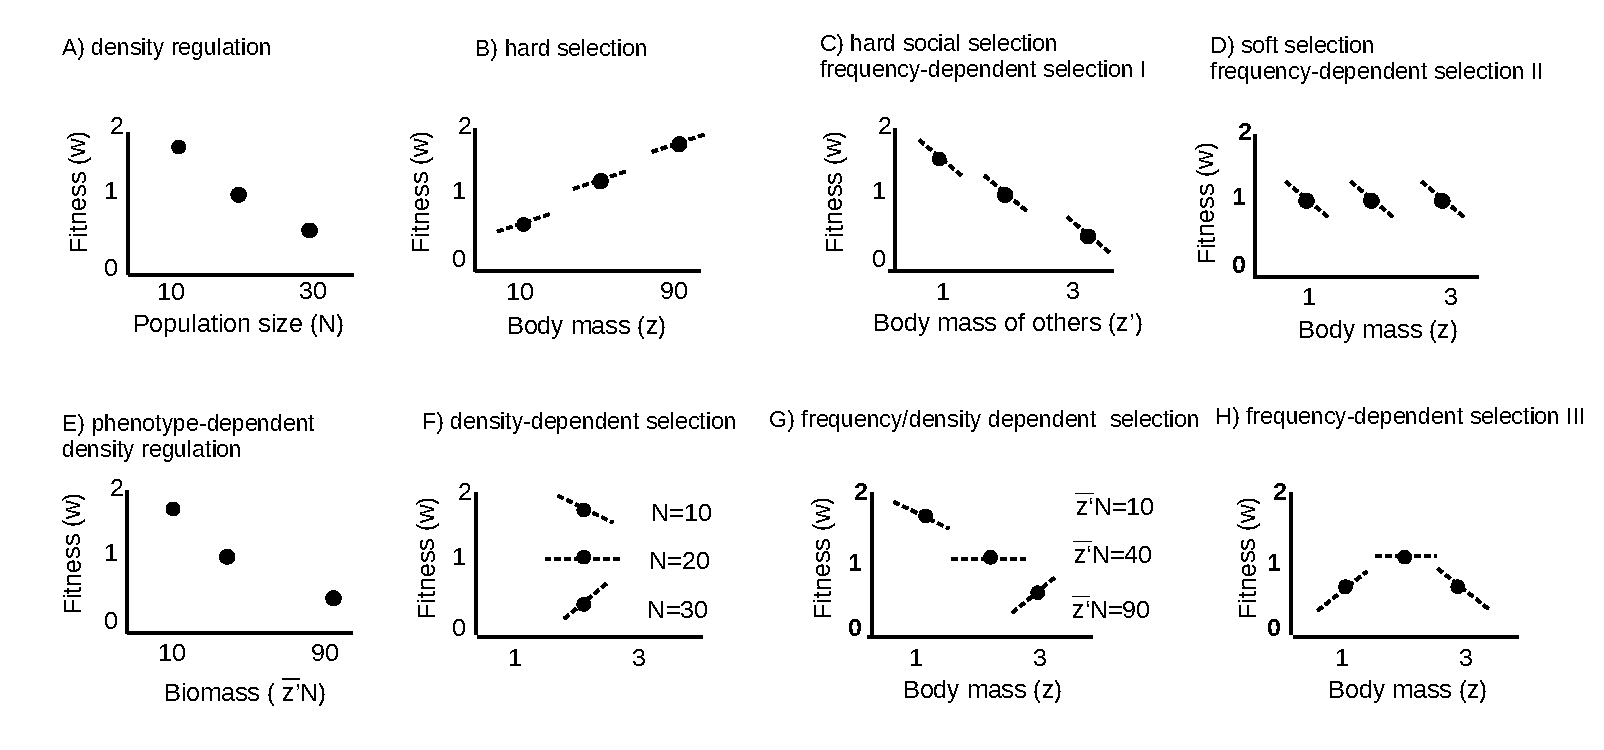
\includegraphics[width=15cm, height=7cm]{Figures/Fig2.pdf}
	\caption{Social environment effects on the eco-evolutionary dynamics of populations. Here $w$ is used to denote the fitness of individuals, $z$ their phenotypes, $N$ the number of individuals in the population, and $z’$ the phenotypes of other individuals in the population. While $\bar{z'}$ represents the average phenotype in the social environment. Black dots represent the average phenotype $\bar{z}$ and fitness $\bar{w}$ for a selection episode, and dashed lines represent the phenotype-fitness relationship within each selection episode. (A) Density regulation, where the number of individuals ($N$) affects the fitness ($w$) of all individuals independent of phenotype. (B). Hard selection where the relationthsip between an individual's phenotype and its own fitness is independent of the social environment (i.e frequency and density independent).  (C) Hard social selection (frequency-dependent selection I), where the phenotype (body mass) of other individuals in the population ($z'$) affects individual absolute fitness ($w$), causing that the mean phenotype in the social environment to affect the size of population through its (hard selection) effects on mean fitness. (D) Soft selection, where the fitness  of a phenotype is relative to the phenotype of the individuals with whom it interacts (i.e. dashed lines). (E) Phenotype-dependent density regulation, where the impact an individual has on the absolute fitness of others depends upon its phenotype (i.e. body mass), and so in this scenario the effect of population size on fitness ($w$) is moderated by the average phenotype in the population ($\bar{z'}N$). (F) Density-dependent selection, where the within-episode relationship between an individual's phenotype ($z$) and its absolute fitness ($w$) depends upon the number of individuals in the population ($N$) but not on the mean phenotype in the population. (F) Density- and frequency-dependent selection, where the within-episode relationship between an individual's phenotype ($z$) and its absolute fitness ($w$) depends upon both the number of individuals ($N$) and the mean phenotype in the population ($\bar{z}$). (G) Frequency-dependent selection III, where the relationship between an individual's phenotype and its absolute fitness ($w$) depends upon the mean phenotype in the population ($\bar{z}$), but is independent of the number of individuals in the population ($N$).} \label{fig:selection}
\end{figure}

\newpage
\begin{figure} [H]
	\centering
	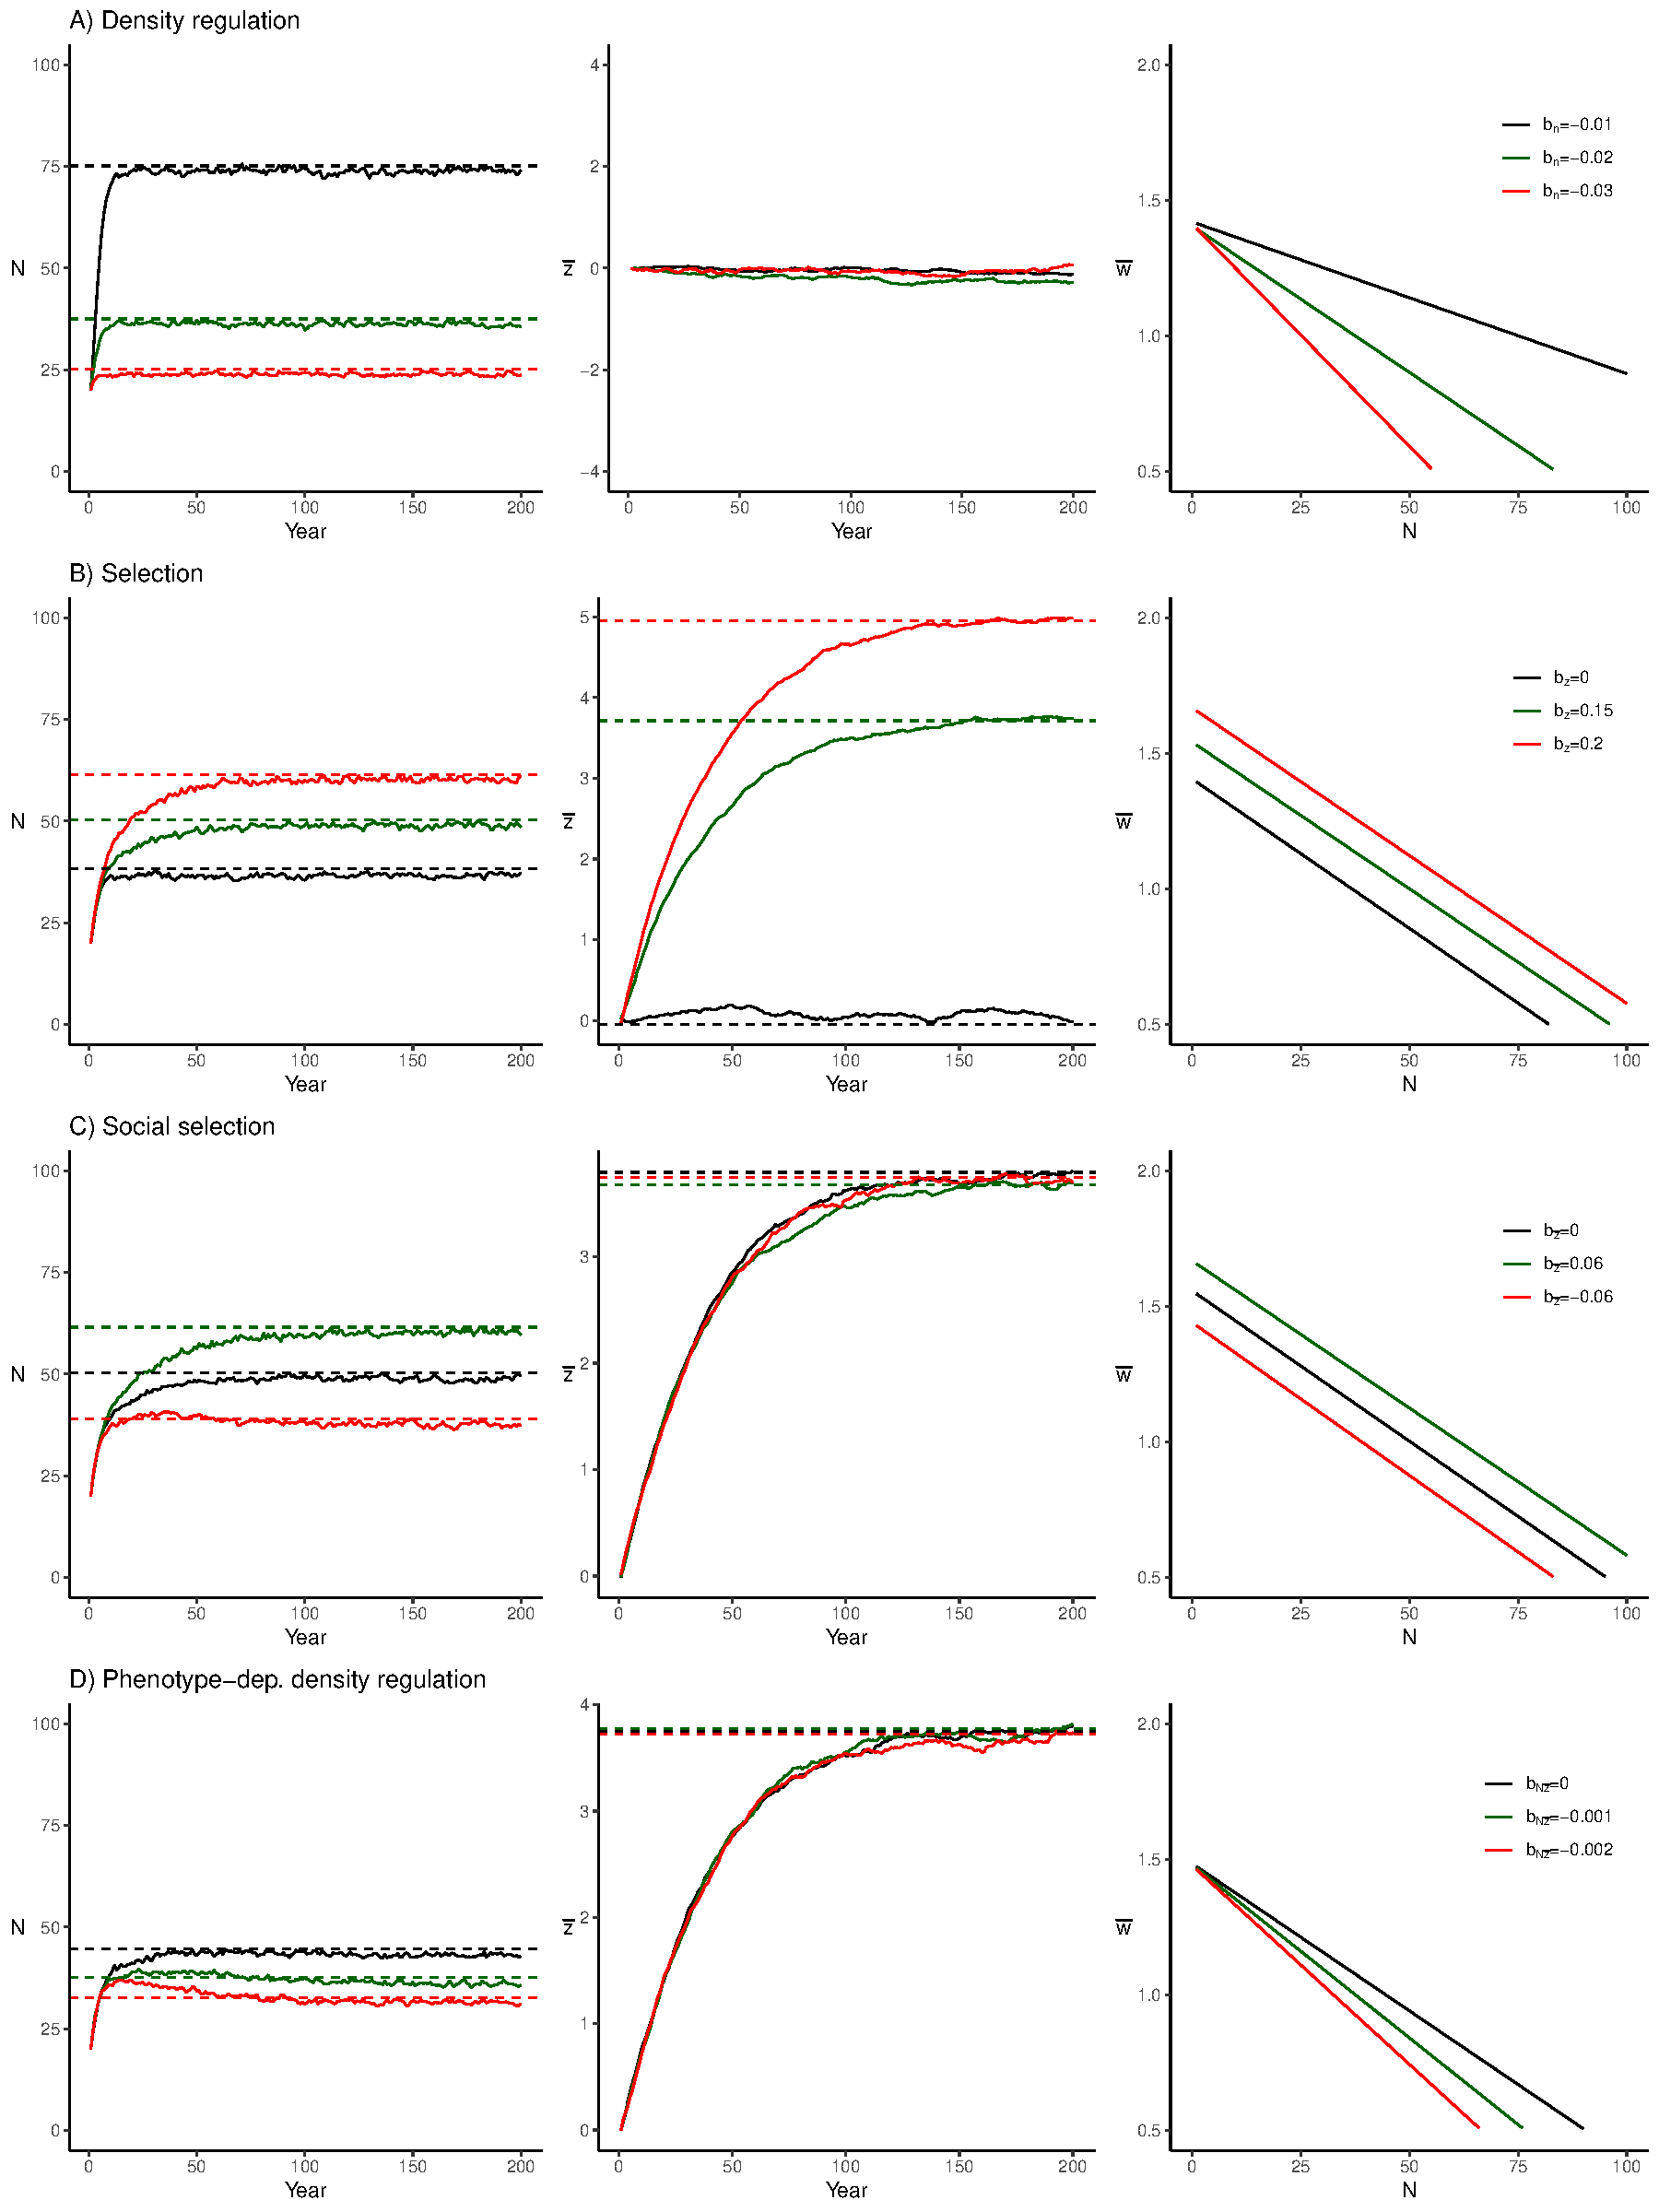
\includegraphics[width=12cm, height=16cm]{Figures/Fig3.pdf}
	\caption{Individual-based simulations results for scenarios 1-4 involving density regulation, direct selection on the phenotype, 'hard' social selection and phenotype-dependent density regulation. The left-hand graphs show the trajectory of population size (N) each Year until it arrives at its equilibrium, the middle graphs show the trajectory of the mean phenotype ($\bar{z}$) each Year evolving towards its equilibrium, and the right hand graphs show mean fitness ($\bar{w}$) as a function of population size (N). In each scenario we varied a specific parameter while keeping the others constant (see Table 2 for details of simulation parameters). The values for the parameters that were changed in each case are presented in the legends in the right-hand graphs. Hence the lines of different colours represent different parameter values for each scenario, and horizontal dashed lines of each colour are the equilibrium population sizes and mean phenotypes predicted from the statistical model estimates. (A) A scenario with only density regulation and no selection on the phenotype (i.e. where the average phenotype of the population matches the optimum phenotype and there is no phenotypic evolution - see middle graph). The strength of density regulation (colour-coded changes in $b_n$ depicted in the right-hand graph) results in different equilibrium population sizes (left-hand graph). (B) A scenario with direct selection on the phenotype (e.g. the introduction of a new resource resulting in selection for the ability to exploit it), where the different coloured lines represent different strengths of directional selection ($b_z$) on the phenotype. Evolution gradually shifts the mean phenotypic values closer to the equilibrium phenotype (middle graph), resulting in different equilibrium population sizes (left-hand graph), despite the slope of the effect of population size on mean fitness being the same throughout (right-hand graph). (C) A scenario where the phenotype of individuals in the social environment affects individual absolute fitness, with different strengths of 'hard' social selection or frequency-dependent selection I ($b_{\bar{z}}$). This affects the equilibrium size of the population (left-hand graph) because it influences the mean fitness of the population (different elevations in the right-hand graph), even though the equilibrium phenotype remains the same (middle graph). (D) A scenario where the effect of population size on average individual fitness depends upon the mean phenotype in the population, with different degrees of phenotype-dependent density regulation ($b_{N\bar{z}}$). Populations with the same mean phenotype (middle graph) can have different equilibrium population sizes (left-hand graph) when the relationship between population size and mean fitness depends on how the mean phenotype modulates the strength of density regulation (i.e. the slope in the right hand graph).}
	\label{fig:sim2}
\end{figure}
\newpage
\begin{figure} [H]
	\centering
	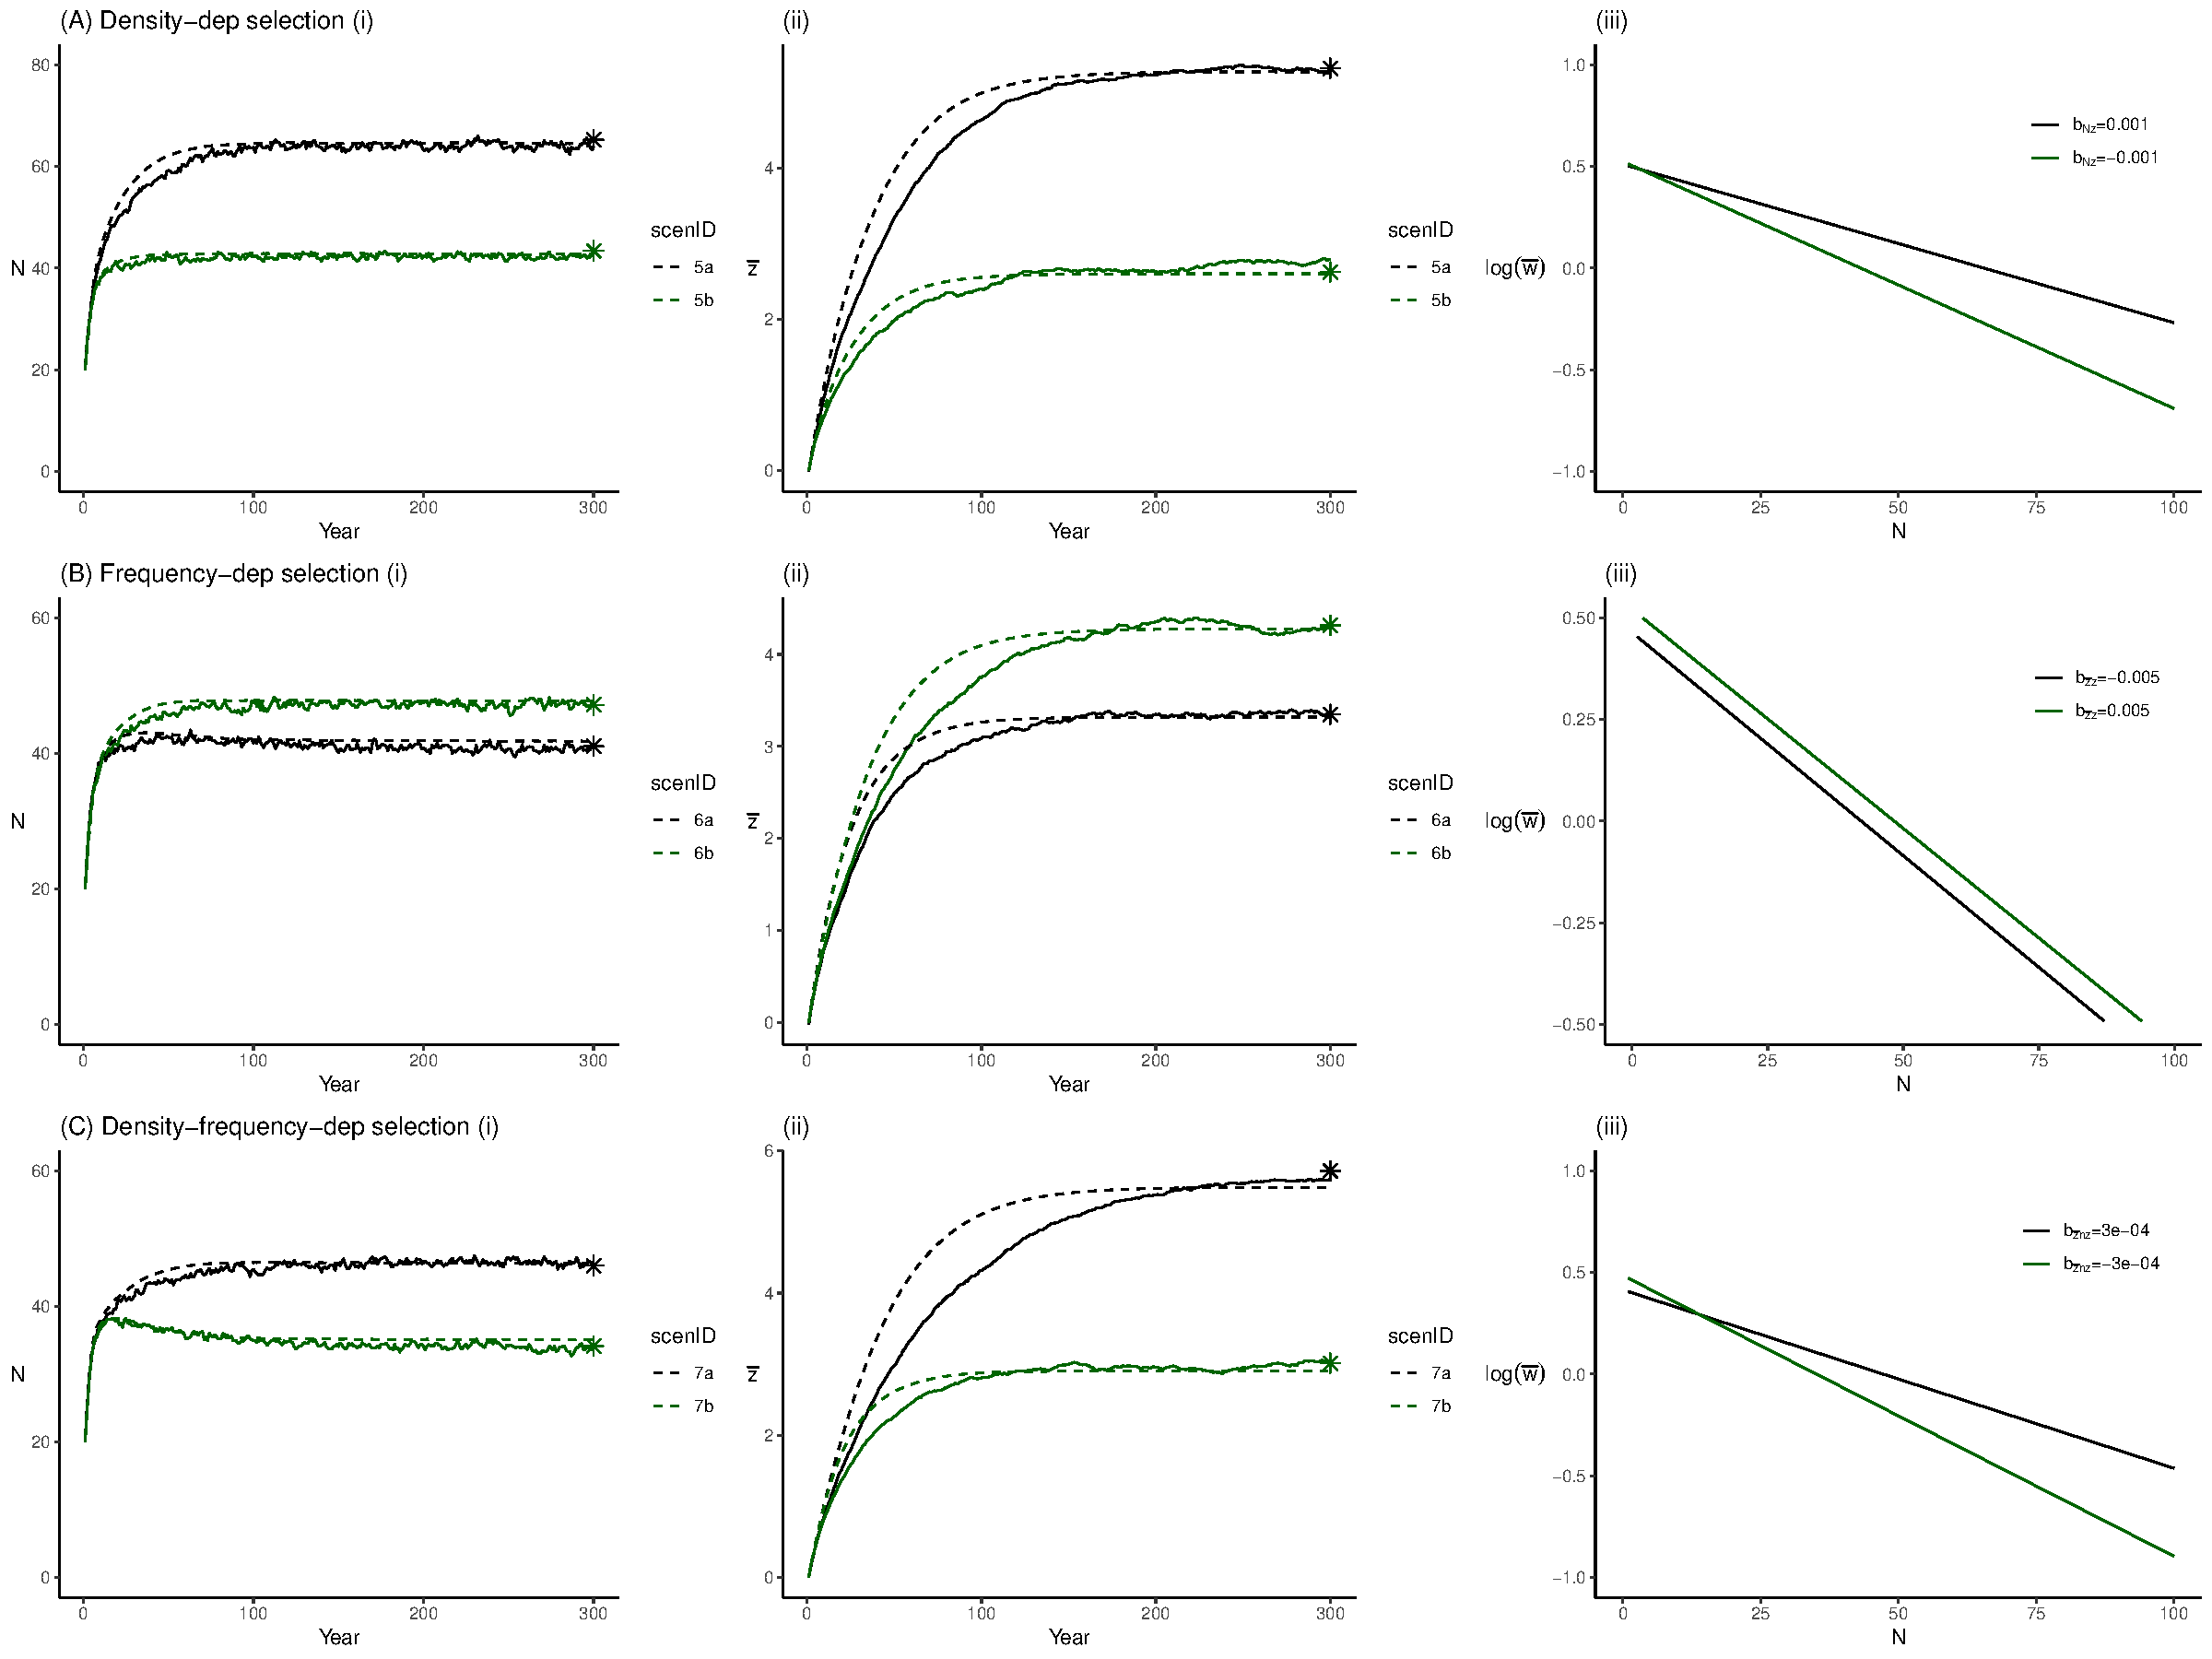
\includegraphics[width=12cm, height=12cm]{Figures/Fig4.pdf}
	\caption{Individual-based simulation results for scenarios 5-7 showing the eco-evolutionary consequences of density-dependent selection (A), frequency-dependent selection II (B), and their interaction (C). As in Figure 3, the left-hand graphs show the trajectory of population size over time, the middle graphs the trajectory of the mean phenotype, and the right-hand graphs the relationship between population density and mean fitness. Coloured lines represent different parameter values for each scenario, and horizontal dashed lines are the equilibrium population size and mean phenotype predicted from these using the statistical estimates. (A) Scenario 5 varied the density-dependent selection coefficient $b_{zn}$ to show how this alters the strength of density regulation (the slope in the right-hand graph), with direct consequences for the equilibrium population size (left-hand graph) and the mean phenotype (middle graph).(B) The frequency-dependent selection II scenario 6 varies the coefficient $b_{\bar{z}z}$ to demonstrate the consequences for the equilibrium phenotype as well as the population size via the effect of the mean phenotype on mean fitness (with no affect on the strength of density regulation - right-hand graph). (C) Scenario 7, when these two processes (A and B) interact resulting in frequency- and density-dependent selection, where the strength of the  coefficient ($b_{\bar{z}nz}$) will determine the interdependence between the mean phenotype and the equilibrium size of the population. The strength of this coefficient will affect both the mean fitness of a population when its size is very small (the intercept) and how population size affects the mean fitness of the population (the slope) of  the left-hand graph, which can result in a variety of different effects on the equilibrium population size and mean phenotype (see Figure 5).} 
	\label{fig:sim3}
\end{figure}
\newpage
\begin{figure}  [H]
	\centering
	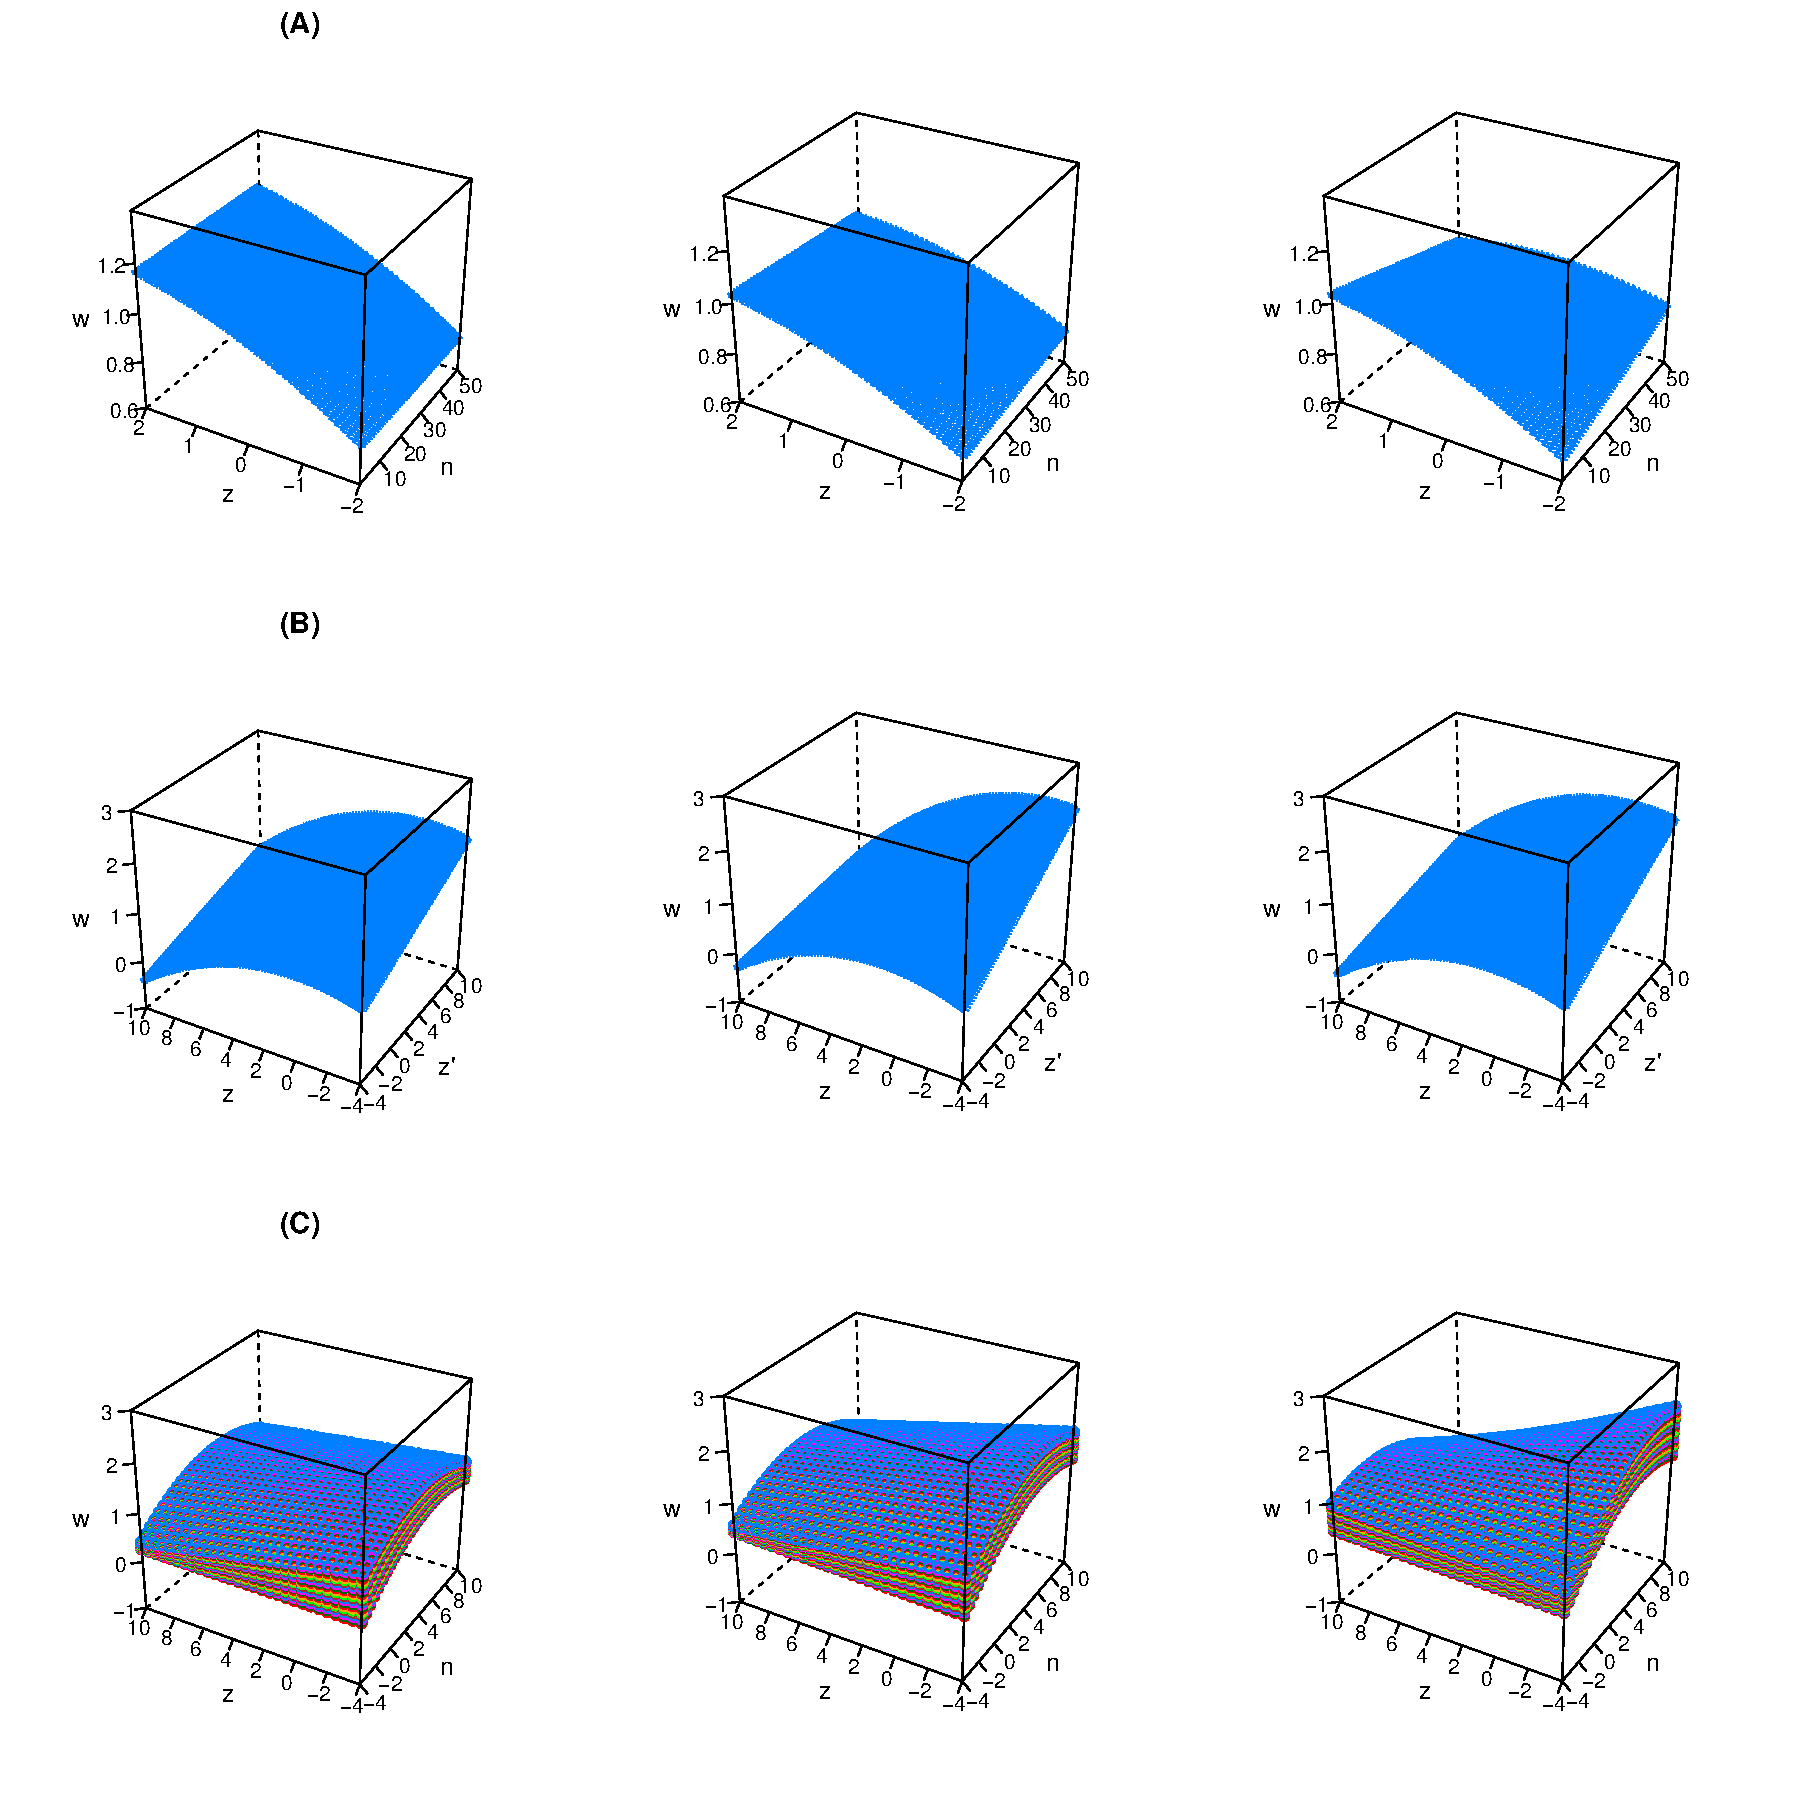
\includegraphics[width=12cm, height=12cm]{Figures/Fig5.pdf}
	\caption{Fitness surfaces for different scenarios 5 density-dependent selection (A), 6 frequency-dependent selection (B), and 7 frequency- and density-dependent selection (C). Surfaces show relative fitness to emphasize the effects on selection within each episode. The fitness surfaces corresponds to the predictions based upon the multiple regression estimates. Each column represents a different set of simulations with different parameter values for each scenario (see Table 2; Figure 4). In (C) the different colours represent a different mean phenotype. In this scenario 7, the fitness surface describing the relationship between an individual's phenotype, its fitness and the average phenotype in the social environment changes depending upon the size of the population.} 
	\label{fig:surface}
\end{figure}


\newpage

\section{Text boxes}

\subsection{Box 1: Social interactions mediate eco-evolutionary feedbacks}

\noindent Figure 1 depicts the role of social interactions in mediating eco-evolutionary feedbacks through density- and frequency-dependent processes \citep{Engen2020}. Path 1 (p1) shows how the strength of competition for limited resources determines population size through density regulation \citep{Gilpin1973a}. Change in population size in turn affects density-dependent competition (p2), creating the classic ecological feedback (p1,2) determining the equilibrium size of a population \citep{Travis2013}. If selection is density-dependent (p1,2,3), the size of a population will also have cascading effects on phenotypic selection  \citep{Mueller1997, Boyce1984}. For instance, when populations are large and closer to carrying capacity, investing in somatic growth and competitive behaviours to monopolize resources may be favored. In contrast, when populations are small and resources are abundant, selection may favor smaller individuals that invest in rapid reproduction instead of body size and longer-term competitive ability \citep{Joshi2001, Wright2018, Engen2017}. Density-dependent selection may thus result in the optimal phenotype being dependent upon population size \citep{Anderson1971, Charlesworth1971}. Evolutionary adjustments in the population mean phenotype can, in turn, influence the strength of competitive interactions via the relative frequencies of different phenotypes in the population \citep{Wright1969} (p4,1). Following the example of body size, as competition increases the average individual becomes larger and needs more resources, thus reducing the maximum possible size or carrying capacity of the population \citep{Engen2020}. However, evolution may instead favor social strategies that maximize efficiency of resource use in order to ameliorate the negative fitness effects of competition, potentially increasing the carrying capacity of such populations \citep{macarthur1967theory,  Boyce1984}. When the fitness payoffs of a competitive strategy depends on the strategy of other individuals in the population, the average phenotype in the population can also influence the optimal phenotype for a given individual. This will cause frequency-dependent selection, further affecting both phenotypic evolution (p4,3) \citep{Heino1998} and population size (p4,3,1) \citep{Svensson2018}. Social interactions thus mediate the feedback between ecological and evolutionary dynamics, linking the evolutionary stable phenotype with the equilibrium size of a population (p5).

\begin{figure}[H]
	\centering
	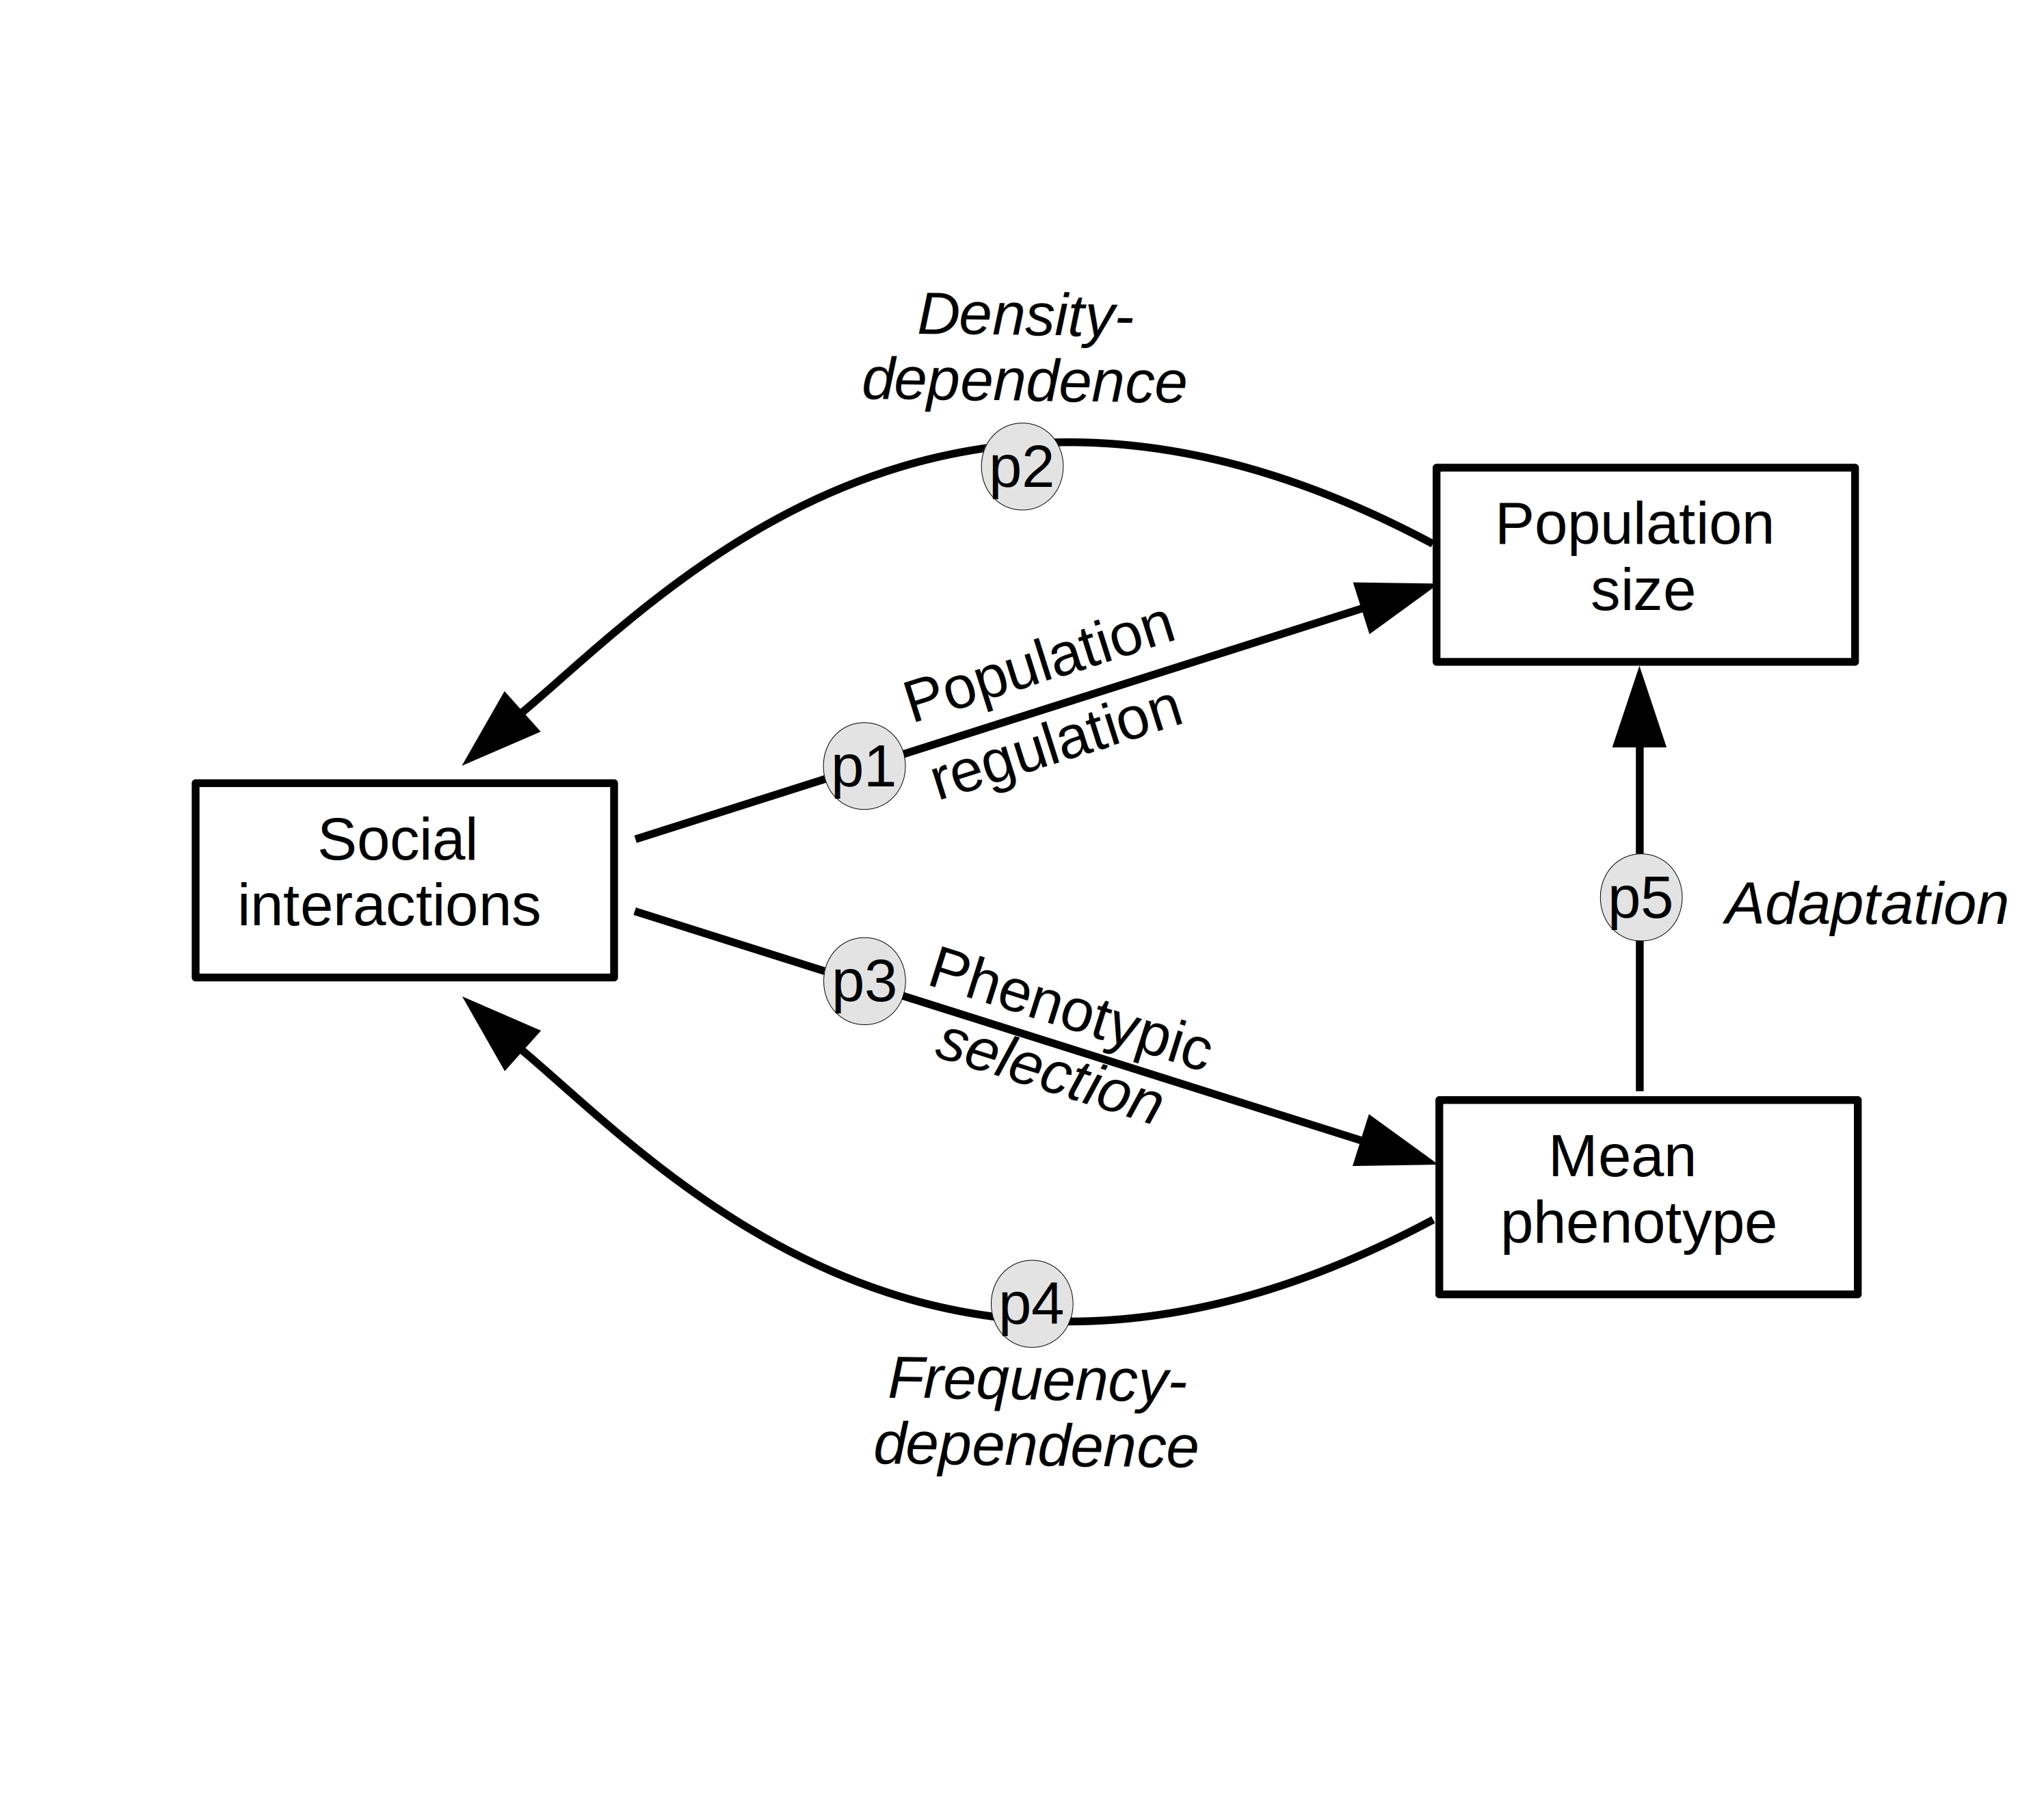
\includegraphics[width=8cm, height=7cm]{Figures/Fig1.jpg}
	\caption{Social interactions mediate eco-evolutionary feedbacks}
\end{figure}


\newpage
\subsection{Box 2: The many types of frequency dependent selection} 
\noindent Theoretical models developed in population genetics \citep{Fisher1930, Wright1969}, game theory \citep{MaynardSmith1982, McGill2007, McNamaraLeimar2020} and quantitative genetics \citep{Lande1976, Lande2007, Engen2020} have demonstrated how frequency-dependent selection can affect phenotypic evolution. Classic examples include Fisher's runaway model of sexual selection and the evolution of stable sex ratios \citep{Fisher1930}. Frequency-dependent selection is used to describe many different processes and its definition has been extensively discussed, specially in the context of population genetics and the maintenance of polymorphisms \citep{Ayala1974, Gromko1977, Heino1998}. All the uses of frequency-dependent selection have in common that the fitness of a phenotype varies with its frequency in the population. However, it is useful to make the distinction between the different types of frequency-dependent selection as they have different consequences for phenotypic evolution and population dynamics. Here we distinguish them from a statistical perspective based on whether the effects of the individual's phenotype and that of its social environment on its fitness are additive (frequency-dependent selection I), relative (frequency-dependent selection II) or interactive (frequency-dependent selection III).

We refer to frequency-dependent selection I (Figure B2.i \& ii) to scenarios in which the effect of the average phenotype in the social environment, and the effect of individual's phenotype on its own fitness have additive effects ($\beta_z \mathbf{z} + \beta_{\bar{z}} \mathbf{\bar{z}}$ ). This scenario has been shown to result in maladpation \citep{Lande1976} and thus affect population dynamics \citep{Lande2007}. We described this scenario in the main text as hard social selection (Figure 2C), because the direct effect of an individual's phenotype on fitness does not change as a function of the average phenotype in the social environment, affecting the absolute fitness of individuals. We use the term frequency-dependent selection II to describe scenarios in which the the effect of a phenotype on fitness is relative to the average phenotype in the social environment ($\beta_z [z-\bar{z}]$). This type of frequency dependent selection includes soft selection (Figure 2D), which was described to be frequency and density dependent in its inception, but it was suggested to have little effect on population dynamics \citep{Wallace1975, Bell2021}. This can be thought of as a zero-sum game, where a fitness gain of one indivdiual, results directly in the a fitness loss in another individual, and thus soft selection has no effect on the mean fitness in the population. Frequency-dependent selection II can also be related to the more narrow definitions that require (negative) frequency-dependent selection to result in the stable coexistence of polymorphisims (i.e. where the fitness of a phenotype decreases with its relative frequency in the population). This process was in the center in the early developments of the concept of frequency-dependent selection in population genetics \cite{Gromko1977, Ayala1974, Heino1998}. In a quantitative genetic framework, it can formulated as a type disruptive selection \citep{Burger2004}, were the effects of a phenotype depends on the absolute deviation from the average phenotype in the population ($z-\bar{z}^2$). We refer to frequency-dependent selection III (Figure 2G) to scenarios in which an individual's phenotype interacts with the average phenotpye of its social environment to affect its fitness ($\beta_{z\bar{z}} \mathbf{\bar{z}z}$). This results in a wrapped fitness surface were the direct effect of a phenotype on fintess changes with the average phenotpye in the social environment (Figure B2.v \& vi). This may represent a type of balancing selection \citep{Gromko1977}. For instance a scenario were the mean phenotype becomes larger the smaller phenotype has an advantage, but as the mean phenotype becomes smaller the larger phenotype has an advantage.

\begin{figure}[H] 
	\centering
	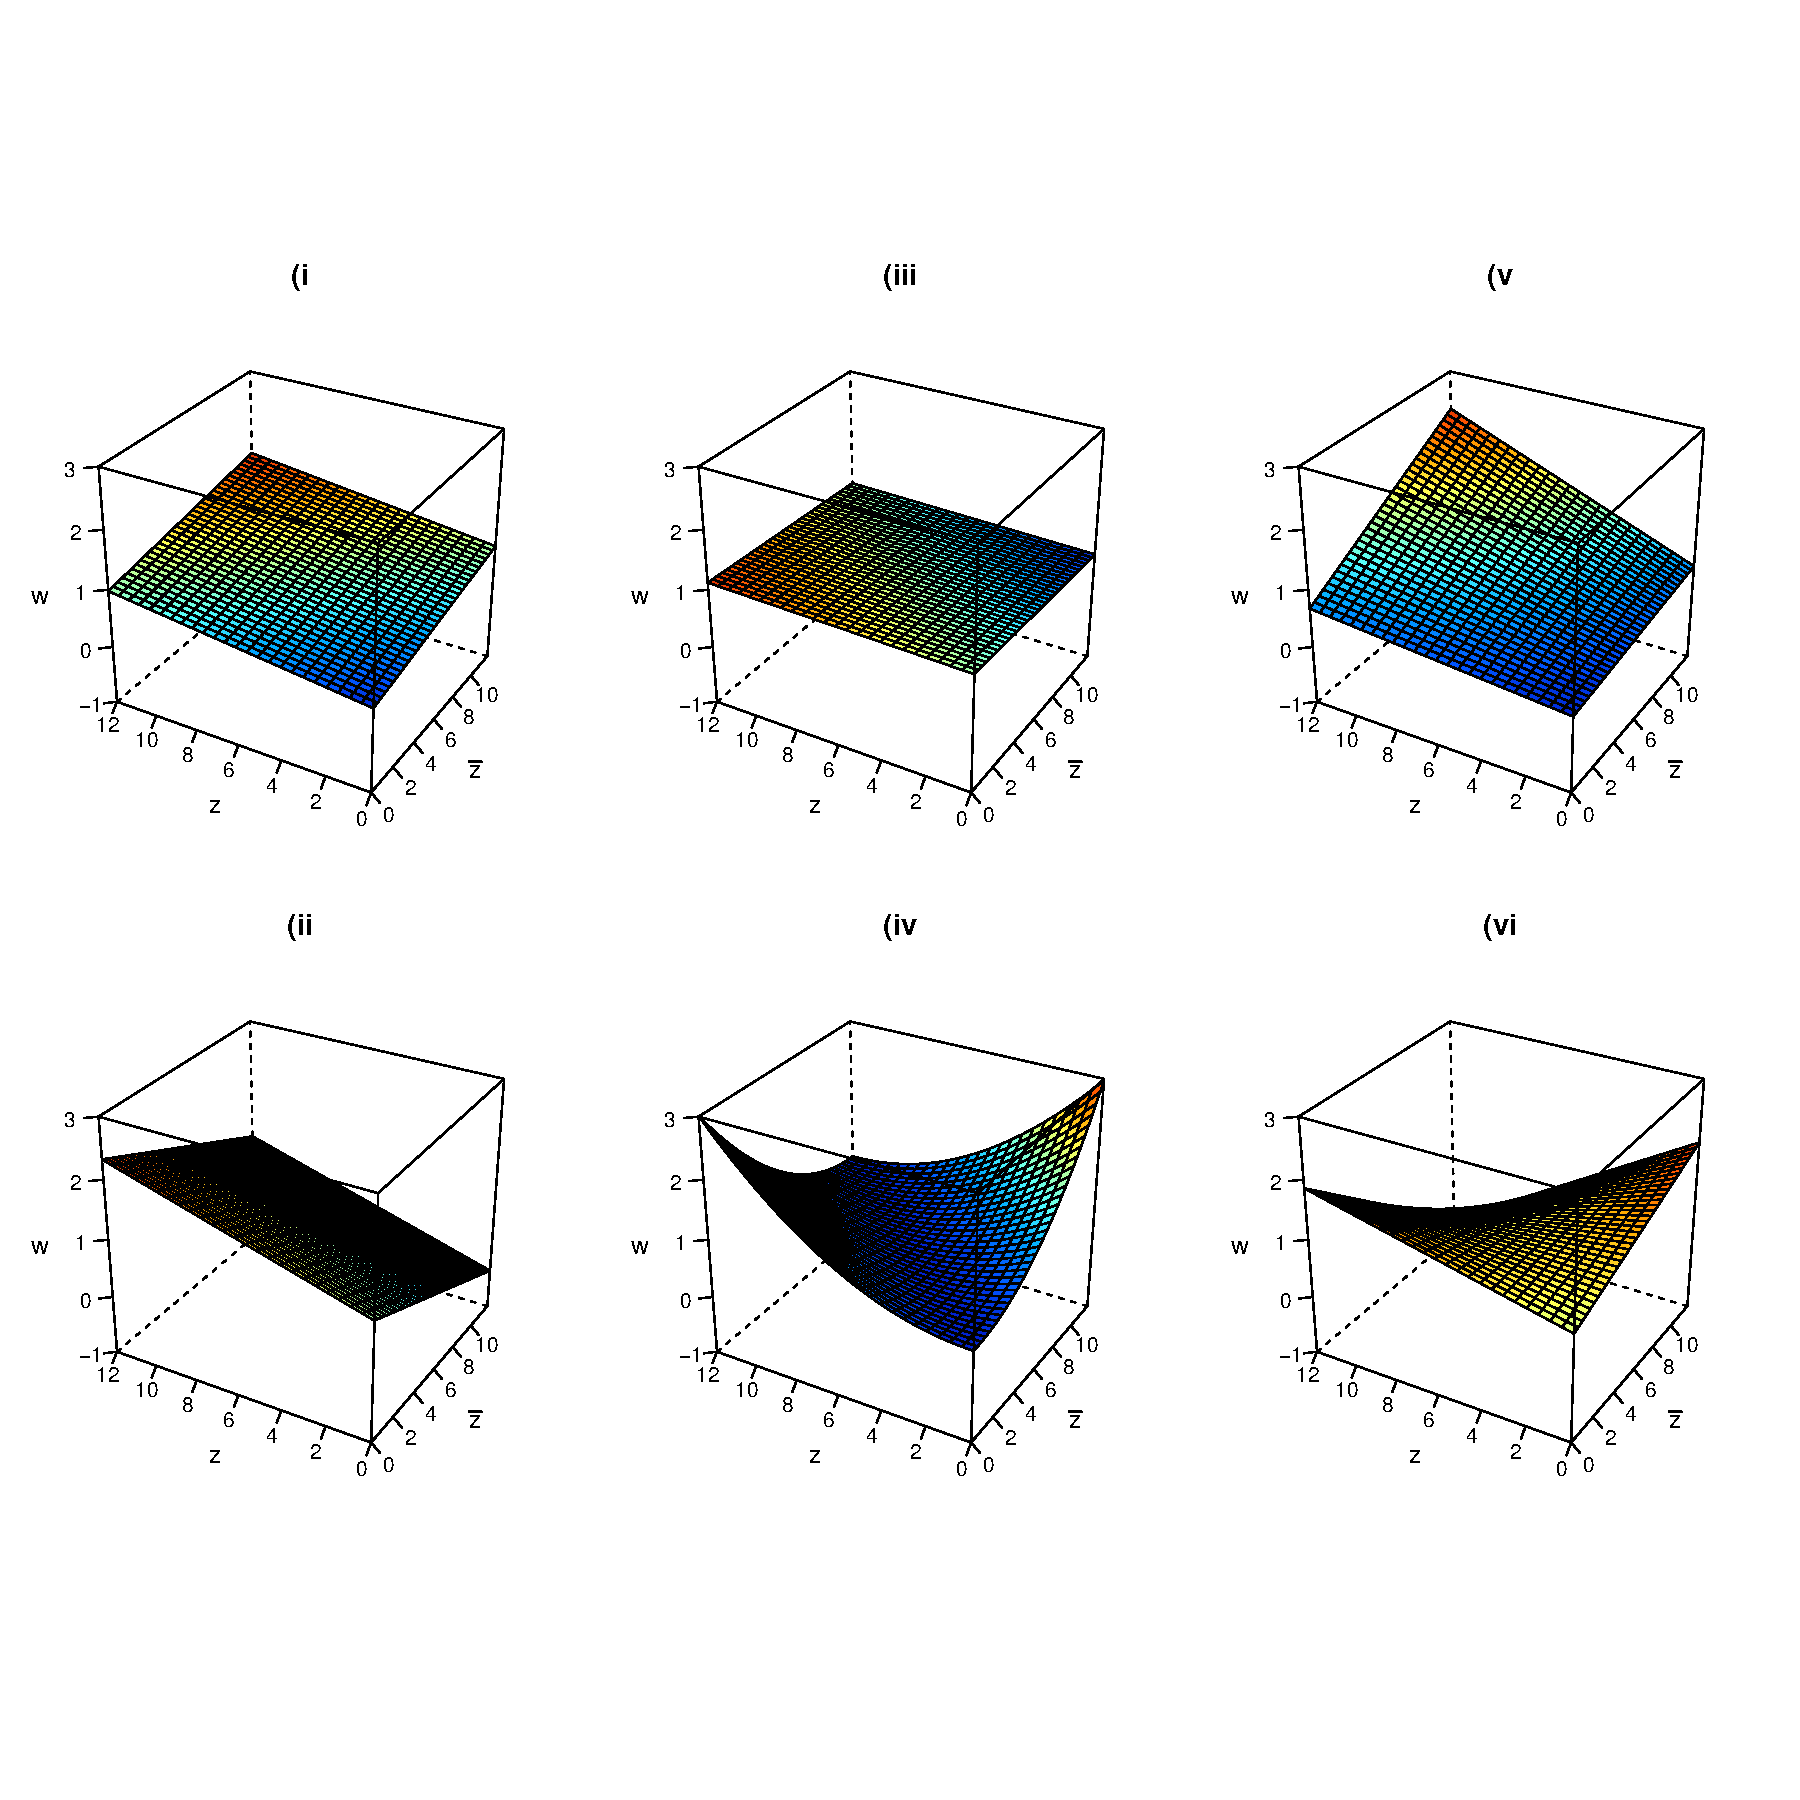
\includegraphics[width=14cm, height=14cm]{Figures/Box2.pdf}
	\caption{Fitness surfaces for different types of frequency dependent selection. i)  represents scenarios of postive and negative i) frequency dependence I in which the effects of an indvidual's phentopye and that of its social environment have additive effects on its fitness. iii \& iv) represents scenarios of frequency-dependent selection II in which the effects of an indvidual's phentopye on its fitness is relative to the average phenotype of its social environment. iii) Depicts a scenario of positive selection for having a higher phenotype that that of the average individual in the social environment ($z-\bar{z}$). iv) Represents scenarios of negative- frequency dependent selection in which the effects of a phenotype depends of the absolute deviation from the phenotype of the individuals in the social environment $(z-\bar{z})^2$). v) represent scenarios of negative and positive vi) of frequency dependence III in which an individual's phenotype interacts with that of its social environment to affect its fitness. In this scenarios the fitness function depends on the mean phenotype in the social environment.}
	\label{fig:Box2}
\end{figure}


\subsection{Box 3: An eco-evolutionary individual-based simulation}
We used individual-based eco-evolutionary simulations to study how selection and density regulation interact to determine a population's equilibrium size and mean phenotype. For simplicity we only focus on the females of an asexual population of size $n_{1}$, which is a common when studying population dynamics. We simulated a set of scenarios reflecting how social interactions may affect the equilibrium size and mean phenotype of populations. The number of recruits an individual produces $bm{r_{t}}$ is simulated as a Poisson process depending upon density regulation, an individual's phenotype, the phenotype of the individuals in the social environment and their interactions. Adult survival from one given year to the next ($\bm{s}$) is modeled as a Bernoulli process. For simplicity, we assume that survival is not affected by an individual's phenotype or its social environment. Thus the average survival propensity ($\bar{p}$) defines the survival probability for all adult individuals across all breeding episodes. The population size the next year ($n_{t+1}$) is a function of the individuals that survive plus the new recruits produced by individuals breeding in the previous generation, $n_{t+1}=\sum \bm{s_{t}} + \bm{r_{t}}$. To simulate a range of different scenarios, we focus on an increasingly complex subset of parameters aimed at capturing different social processes affecting the reproduction of individuals. The full equation capturing the processes affecting the survival and reproduction of individuals in a given year is:

\begin{subequations} 
	\begin{gather}
	\bm{r}\sim Poisson(e^{R_{0} + b_{n} \bm{n} + b_{z} \bm{z} + b_{q} \bm{z^2} + b_{\bar{z}} \bm{\bar{z}} + b_{n \bar{z}} \bm{n\bar{z}} + b_{z\bar{z}}  \bm{z\bar{z}} + b_{zn}  \bm{zn} + b_{zn \bar{z}} \bm{zn\bar{z}}+  \bm{e}}), \label{eq:Full1a} \\
	\bm{s}\sim Bern(\frac{1}{e^{\bar{p}}}). \label{eq:Full1b}
	\end{gather}
\end{subequations}

 In all scenarios, the number of offspring produced by an individual that recruit to the next generation in a given year is a function of the average population-level reproduction when population size is very small, $R_0$, and any population size effects on mean fitness described by the density regulation coefficient $b_{n}$. The first scenario (S1) solely focuses on how different strengths of density regulation result in different equilibrium population sizes (depicted in Figure 2A). In scenario (S2), the number of recruits an individual produces is affected by its own phenotype as a function of the linear ($b_z$) and quadratic ($b_q$) effects of the phenotype on fitness. In this scenario we varied the strength of directional selection ($b_z$) to show how it results in different equilibrium phenotypes.The next scenario (S3) represents situations were the number of recruits produced by an individual not only depends upon its own phenotype, but also upon the (average) phenotype ($\bar{z}$) of the other individuals in the population (figure \ref{fig:selection}C), as a function of the coefficient $b_{\bar{z}}$. In the next scenario (S4), the fitness of an individual is further affected by the average phenotype of the individuals in the population ($\bar{z}$) in combination with the number of individuals ($n$) in the population (depicted in Figure 2B). This is captured by the interaction coefficient $b_{n\bar{z}}$. We further simulated scenarios where the optimal phenotype in the population depends upon the mean phenotype of the population (S5 Frequency-dependent selection 2, depicted in Figure 2G) by adding the parameter $b_{z\bar{z}}$. Conversely, the optimal phenotype can be made to depend only upon the number of individuals in the population (S6 Density-dependent selection; Figure 2E) by adding the interaction coefficient $b_{zn}$. Finally we model a scenario where the optimal phenotype depends upon an interaction between the number of individuals and the phenotype of the average individual in the population (S7 Frequency- and density-dependent selection; Figure 2F), by adding the parameter $b_{zn\bar{z}}$.
 
 For each simulated scenario, we analyzed the output data of the individual-based simulation as we would empirical data sets. We compared the statistical estimates for the expected size and mean phenotype of the population derived from the multiple regression estimates with the corresponding observed mean phenotype and equilibrium size of the population for each of the individual-based simulations. As might be expected from the effects of 'genetic load' \citep{Lande1996}, the estimates from the statistical models predicted are slightly larger equilibrium population sizes than those produced by the actual simulation models. This is because when a population reaches equilibrium and the average phenotype is equal to the optimum, the mean fitness of the population as a whole is lower than the fitness of the optimal phenotype, due to phenotypic variance ($\sigma^2_z$) causing sub-optimal fitness returns for individuals either side of the optimal mean phenotype. Thus the larger the phenotypic variance, the stronger the deviation between the estimated and observed equilibrium population sizes. This is therefore a function of $\beta_q \sigma^2_z$. For simplicity, we present the equilibrium size equations in the main text without correcting factor for the genetic load, but the estimates presented in Table 2 are those correcting for the genetic load.  

% latex table generated in R 3.6.3 by xtable 1.8-4 package
% Fri Nov 26 13:00:36 2021
\begin{table}[ht]
\centering
\begin{tabular}{lrrrrrrrrr}
  \hline
Scenario & $b_{n}$ & $b_{z}$ & $b_{\bar{z}}$ & $b_{\bar{z}n}$ & $b_{\bar{z}z}$ & $b_{nz}$ & $b_{\bar{z}nz}$ & $\hat{n}_{b}$ & $\hat{z}_{b}$ \\ 
  \hline
(1) Density regulation & -0.02 & 0.00 & 0.00 & 0.000 & 0.000 & 0.000 & 0.0000 & -1.8 &  \\ 
  (1) Density regulation & -0.03 & 0.00 & 0.00 & 0.000 & 0.000 & 0.000 & 0.0000 & -1.1 &  \\ 
   (2) Hard selection & -0.02 & 0.10 & 0.00 & 0.000 & 0.000 & 0.000 & 0.0000 & -1.6 & 0.0 \\ 
   (2) Hard selection & -0.02 & 0.20 & 0.00 & 0.000 & 0.000 & 0.000 & 0.0000 & -1.2 & 0.1 \\ 
  (3) Hard social selection & -0.02 & 0.15 & 0.06 & 0.000 & 0.000 & 0.000 & 0.0000 & -1.0 & -0.0 \\ 
  (3) Hard social selection & -0.02 & 0.15 & -0.06 & 0.000 & 0.000 & 0.000 & 0.0000 & -1.0 & 0.0 \\ 
  (4) Phenotype-density reg. & -0.02 & 0.15 & -0.03 & 0.002 & 0.000 & 0.000 & 0.0000 & -0.3 & -0.0 \\ 
  (4) Phenotype-density reg. & -0.02 & 0.15 & -0.03 & -0.002 & 0.000 & 0.000 & 0.0000 & -1.1 & -0.0 \\ 
  (5) Density-dep. selection & -0.02 & 0.15 & 0.00 & 0.000 & 0.001 & 0.000 & 0.0000 & -1.9 & -0.0 \\ 
  (5) Density-dep. selection & -0.02 & 0.15 & 0.00 & 0.000 & -0.001 & 0.000 & 0.0000 & -1.3 & 0.1 \\ 
  (6) Frequency-dep. selection & -0.02 & 0.15 & -0.03 & 0.000 & 0.000 & -0.005 & 0.0000 & -0.8 & -0.0 \\ 
  (6) Frequency-dep. selection & -0.02 & 0.15 & -0.03 & 0.000 & 0.000 & 0.005 & 0.0000 & -1.9 & -0.0 \\ 
  (7) Freq.-Den.-dep. selection & -0.02 & 0.15 & -0.03 & -0.001 & 0.000 & 0.000 & 0.0002 & -0.3 & 0.4 \\ 
  (7) Freq.-Den.-dep. selection & -0.02 & 0.15 & -0.03 & -0.001 & 0.000 & 0.000 & -0.0002 & -1.3 & -0.1 \\ 
   \hline
\end{tabular}
\caption{Values in the individual-based simulations. Individual recruit production when population sizes were very small was set to 1.1, and the average survival probability was set to 0.475 for all the simulations. For the simulations that included selection (i.e. $b_z$ was not zero), the quadratic component ($b_q$) was set to 0.002. We also present the difference between the long-term mean population size $\hat{n}_{b}$ and mean phenotype  $\hat{z}_b$ in the individual-based simulations versus the estimated values using the multiple regression parameters.} 
\end{table}
 \label{Table 2} [h]


\section{Supplementary Appendix I}
 Initial formal models of density-dependent selection \citep{Anderson1971, Charlesworth1971} were based upon the logistic function of population growth. These models were then extended to describe more general patterns of density-dependent population growth rates \citep{Gilpin1973a} and its consequences for phenotypic evolution \citep{Gilpin1976}. Extensions of the logistic model allowed different growth trajectories for populations with the same carrying capacity (\textit{K}) by introducing an extra parameter, $\theta$ \citep{Lande2003}. If $\theta$ equals 1 then the model is simply the logistic density dependence model, but larger values of $\theta$ indicate stronger density regulation closer to \textit{K}, whereas for lower values of $\theta$ then the maximum population growth rate occurs when N is less than \textit{K}/2. The dynamics of population growth in our individual-based simulations are best approximated by a $\theta$ logistic model with $\theta$ values above 1 (Figure \ref{fig:growth}). These types of population dynamics are characteristic of vertebrates, where populations grow quickly towards their equilibrium size and then population growth ceases rather abruptly, because resource monopolization (e.g. territoriality) tends to mediate competitive interactions in these systems \citep{Gilpin1973a}. 
 
 \begin{figure}[H] 
 	\centering
 	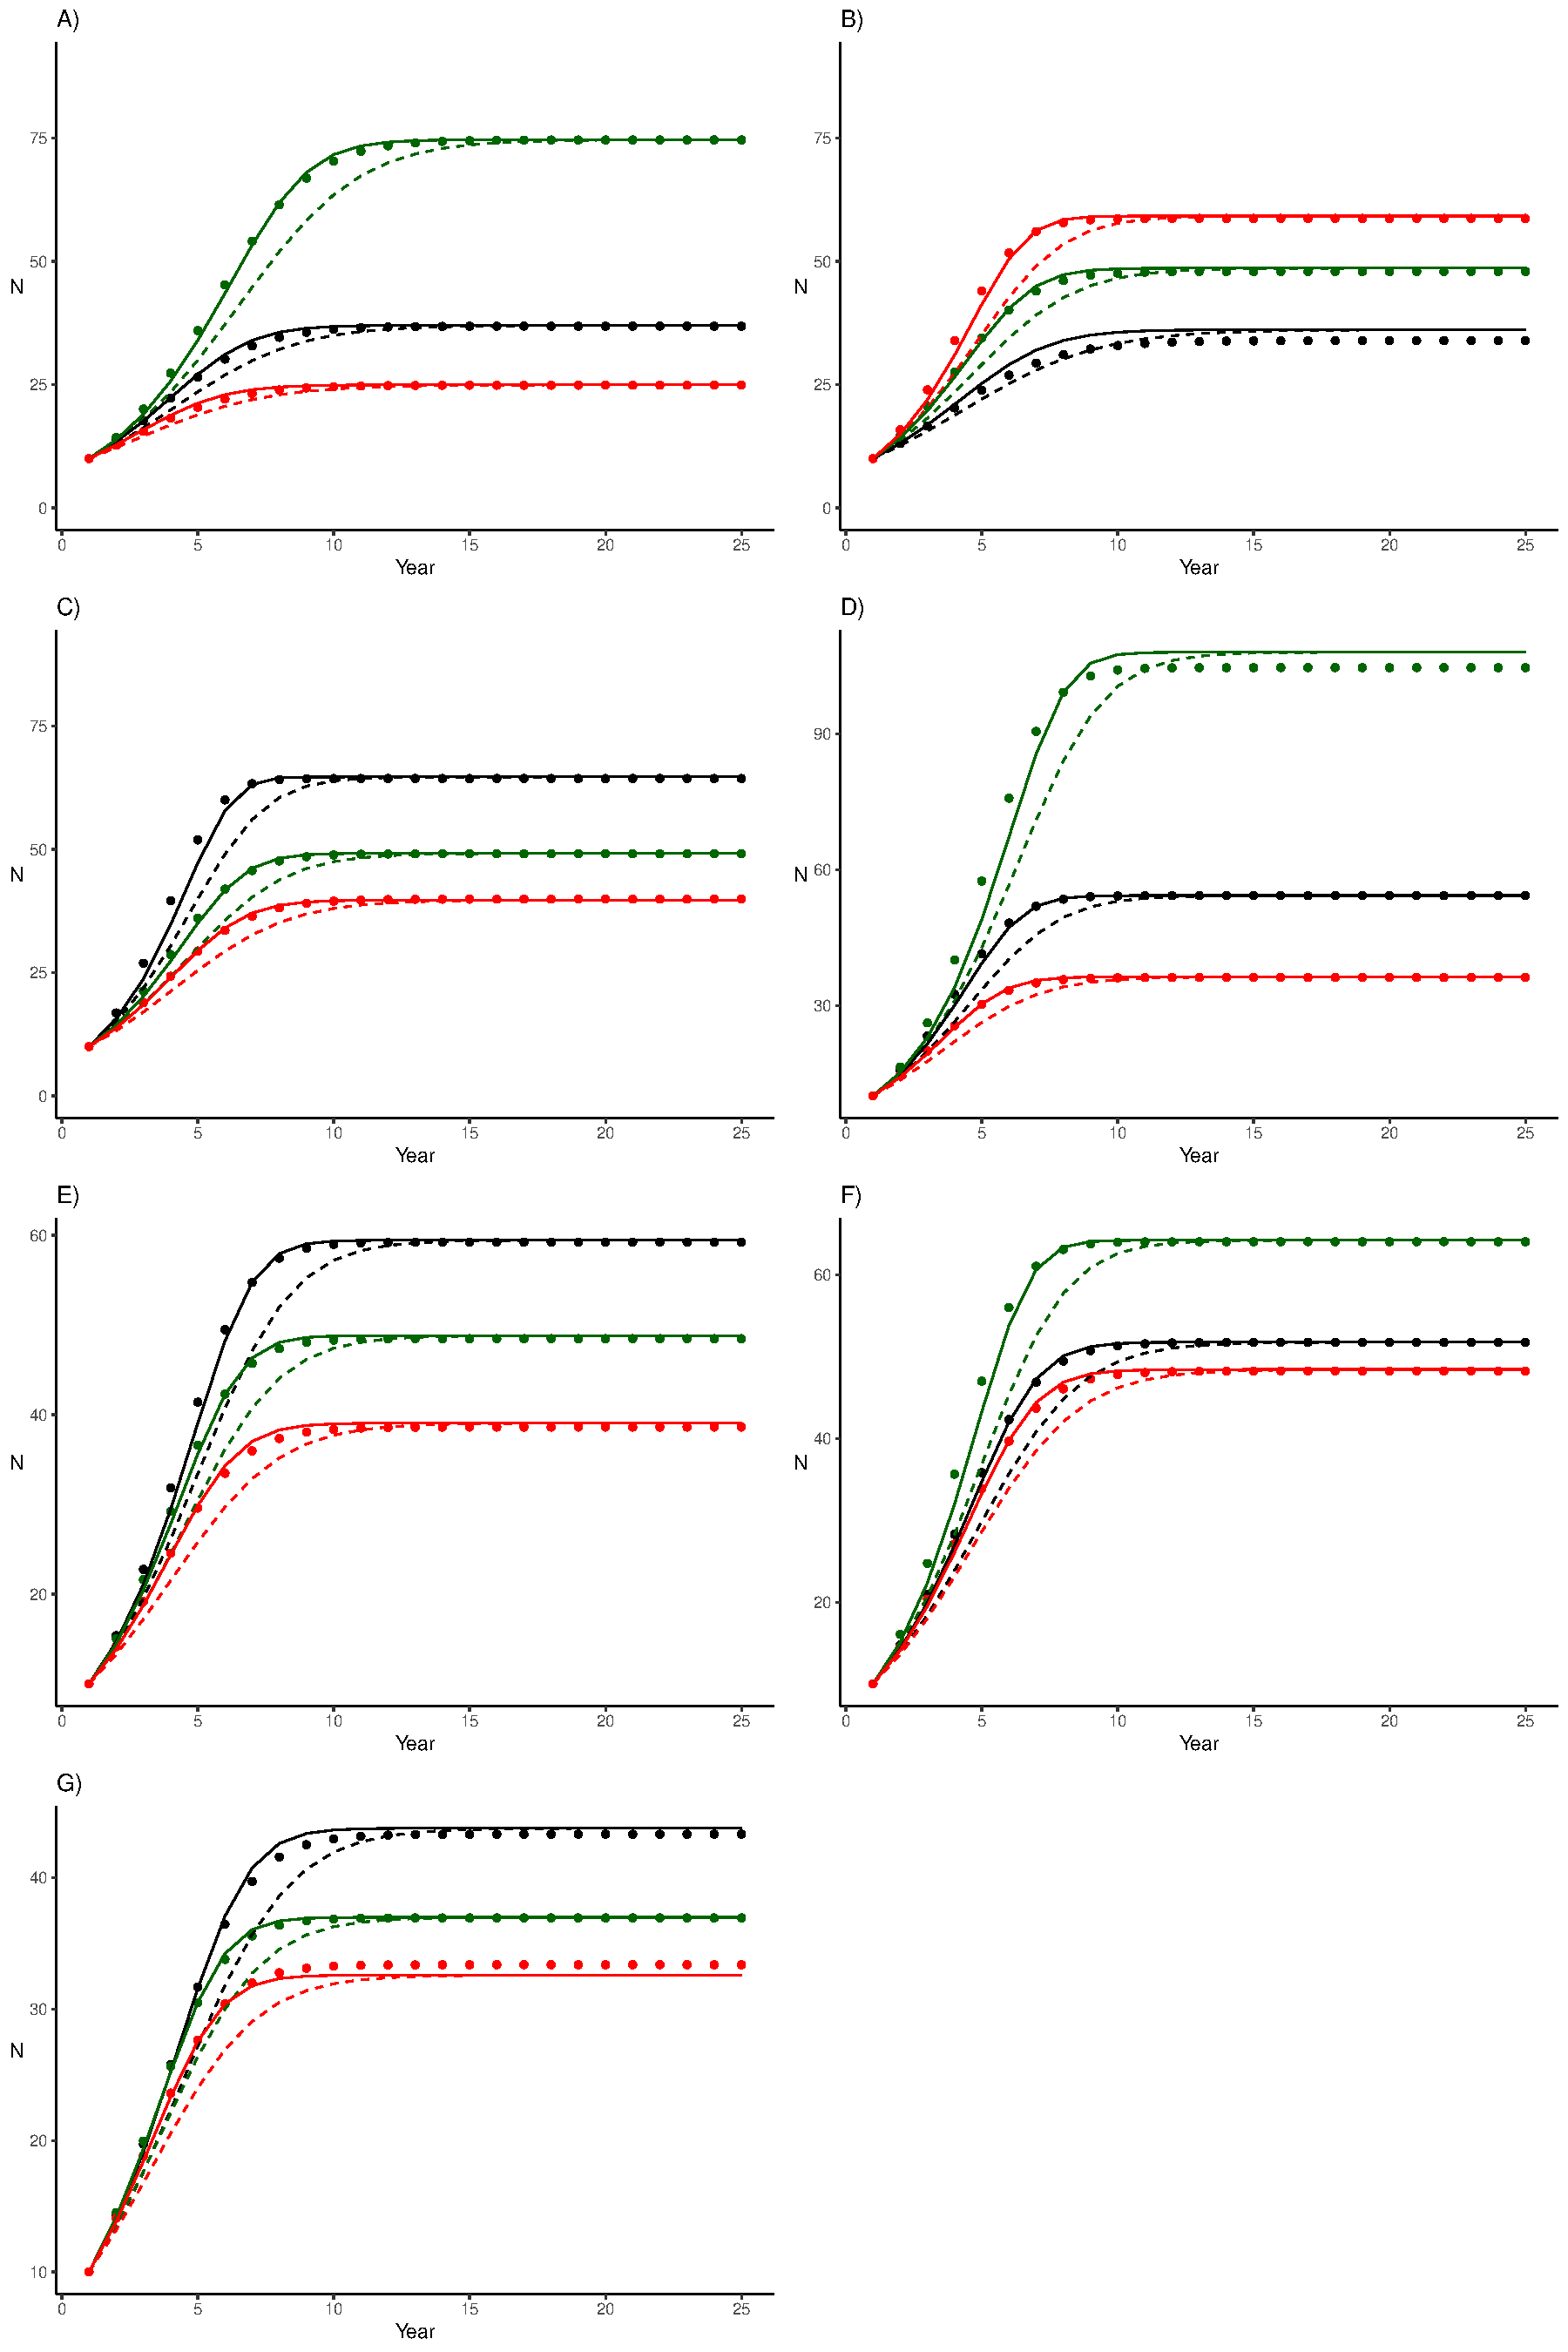
\includegraphics[width=12cm, height=18cm]{Figures/FigS4.pdf}
 	\caption{Predicted changes in population size using the multiple regression estimates (circles), a logistic model (dashed lines) and the theta logistic model of population growth (solid line). Colours represent the different simulations for each scenario (see Table 2). (A) Scenario 1 with density regulation; (B) Scenario 2 with selection; (C) Scenario 3 with social selection; (D) Scenario 4 with phenotype dependent regulation; (E) Scenario 5 with density dependent-selection; (F) Scenario 6 with frequency-dependent selection; and (G) Scenario 7 with frequency- and density-dependent selection.} 
 	\label{fig:growth}
 \end{figure}
 
 \section{Supplementary Appendix II: Ignore from here downwards}
The change in mean phenotype, assuming that the additive genetic variance in the trait is one can be described as:
 
 $$ \Delta \bar{w} = \Delta \bar{w}_{ns} + \Delta \bar{w}_{ed}$$ 
 
 
 $$ \Delta \bar{z} = \beta_{z}. $$ 
 
  $$ \Delta \bar{z} = \frac{1}{\bar{w}} (\beta_{z} + n  \beta_{zn} + \bar{z} \beta_{z\bar{z}} +\beta_{zn\bar{z}} n\bar{z})$$
 
  The changes in the mean fitness of the population associated to hard selection assuming that there is no feedback of its effects on the social environment, in other words assuming the social environment is constant can be expressed as:
 
$$ \Delta \bar{w}_{ns} = \beta_{z} \Delta \bar{z} =  \beta_{z} \frac{1}{\bar{w}} (\beta_{z} + n  \beta_{zn} + \bar{z} \beta_{z\bar{z}} +\beta_{zn\bar{z}} n\bar{z})$$.
 
 This is the change in mean fitness expected by natural selection. However the evolution of the social environment, in terms of its numbers and phenotype, will affect the mean fitness in the population. We can add another term to 
 $$ \Delta \bar{w}_{ed} =   \Delta n\beta_{n} + \Delta \bar{z} \beta_{\bar{z}} + \Delta n \Delta \bar{z} \beta_{n\bar{z}}$$.
 
 $$ \Delta \bar{w}_{ed} =    \beta_{z} \frac{1}{\bar{w}} (\beta_{z} + n  \beta_{zn} + \bar{z} \beta_{z\bar{z}} +\beta_{zn\bar{z}} n\bar{z})[(\bar{w}n-n)\beta_{n\bar{z}}+  \beta_{\bar{z}}] + (\bar{w}n-n) \beta_{n} $$.
 
 $$ \Delta \bar{w} =   \frac{1}{\bar{w}} (\beta_{z} + n  \beta_{zn} + \bar{z} \beta_{z\bar{z}} +\beta_{zn\bar{z}} n\bar{z})(\beta_{z} +  \beta_{n}\bar{w} + \beta_{\bar{z}} + \Delta n \beta_{n\bar{z}})$$.
 
 
 The change in population size is a function of the change in mean fitness, therefore the change in population size also depends on the change in mean phenotype due to hard selection,
 	
 $$	\Delta n = n\Delta \bar{w} = n\beta_{z}\Delta \bar{z} = n\beta_{z}^2 $$
 
The effect of hard selection on number of individuals and the mean phenotype in the social environment will feedbcak on to the population with consequences for the changes in mean fitness. Changes in population size $\Delta n$ and mean phenotype $\Delta \bar{z}$ will feedback to determine equilibrium population size through its effect on the stasis of the mean fitness. This feedback can be described by the coefficients presented in equation \ref{eq: fullw} and the changes in mean phenotype and population size.
 
 \begin{equation} 
 \Delta \bar{w} =  (\beta_{z}\Delta \bar{z}) + (\Delta n\beta_{n} + \Delta \bar{z} \beta_{\bar{z}} + \Delta n \Delta \bar{z} \beta_{n\bar{z}}) + ( \Delta n  \beta_{zn} + \Delta \bar{z} \beta_{z\bar{z}} + \Delta n \Delta\bar{z} \beta_{\bar{z}zn})\Delta \bar{z}.
 \end{equation}
 
 Chages in popultion size and mean phenotype can be further expressed in terms of the coefficients in \ref{eq: fullw}.
 
 \begin{equation} 
 \Delta \bar{w} =  \beta_{z}^2 + (n\beta_{z}^2\beta_{n} +\beta_{z} \beta_{\bar{z}} + n\beta_{z}^2\beta_{z} \beta_{n\bar{z}}) + ( n\beta_{z}^2  \beta_{zn} + \beta_{z}\beta_{z\bar{z}} + n\beta_{z}^2 \beta_{z} \beta_{\bar{z}zn})\beta_{z}.
 \end{equation}
 
 \begin{equation} 
 \Delta \bar{w} =  \beta_{z}^2 + (n\beta_{z}^2\beta_{n} +\beta_{z} \beta_{\bar{z}} + n\beta_{z}^3 \beta_{n\bar{z}}) + ( n\beta_{z}^3  \beta_{zn} + \beta_{z}^2\beta_{z\bar{z}} + n\beta_{z}^4  \beta_{\bar{z}zn}).
 \end{equation}
 
  \begin{equation} 
 \Delta \bar{w} =  \beta_{z} \beta_{\bar{z}} + (1 +n\beta_{n} +  \beta_{z\bar{z}})\beta_{z}^2  + (n\beta_{n\bar{z}} + n \beta_{zn})\beta_{z}^3  +  n  \beta_{\bar{z}zn} \beta_{z}^4.
 \end{equation}
 
 
\end{document}


